\documentclass[12pt]{article}
\usepackage[utf8]{inputenc}
\usepackage[T1]{fontenc}
\usepackage[spanish,es-noshorthands]{babel}
\usepackage{geometry}
\usepackage{graphicx}
\usepackage{xcolor}
\usepackage[pdfauthor={Jorge Giovanni Correa Mejía},
            pdftitle={Justificación Técnica y Económica -- Rehabilitación de Tres Áreas Húmedas},
            pdfsubject={Remodelación Integral de Baños, Bogotá},
            pdfkeywords={remodelación, baños, porcelanato, APU, presupuesto, NSR-10}]{hyperref}
\usepackage[stable]{footmisc}
\usepackage{titlesec}
\usepackage{fancyhdr}
\usepackage{setspace}
\usepackage{enumitem}
\usepackage{booktabs}
\usepackage{longtable}
\usepackage{float}
\usepackage{caption}
\captionsetup[table]{font=small,skip=6pt,labelfont={bf,color=primary},textfont={color=primary!80!black},position=top}
\usepackage{parskip}
\usepackage{ragged2e}
\usepackage[osf]{mathpazo}
\usepackage{eulervm}
\usepackage{microtype}
\SetTracking{encoding={*},shape=sc}{40}
\DeclareMicrotypeSet*{trackingnotes} { encoding = {OT1,T1}, family = {ppl}, series = {bx}, size = {normalsize} }
\usepackage{amsmath}
\usepackage{siunitx}
\sisetup{group-separator={.},group-minimum-digits=4,output-decimal-marker={,}}
\usepackage{pgfgantt}
\usepackage{pdfpages}
\usepackage{tocloft}

\geometry{a4paper, margin=2.5cm, top=3cm, bottom=3cm}

\clubpenalty=10000
\widowpenalty=10000
\displaywidowpenalty=10000

\definecolor{primary}{RGB}{25, 55, 109}
\definecolor{secondary}{RGB}{0, 105, 148}
\definecolor{accent}{RGB}{200, 150, 50}
\definecolor{lightbg}{RGB}{245, 247, 250}

\hypersetup{
  colorlinks=true,
  linkcolor=primary,
  urlcolor=secondary,
}

\setcounter{secnumdepth}{3}
\counterwithin{table}{section}
\renewcommand{\cftsecfont}{\bfseries\color{primary}}
\renewcommand{\cftsubsecfont}{\color{secondary}}
\renewcommand{\cftsecleader}{\cftdotfill{\cftdotsep}}
\titleformat{\section}{\Large\bfseries\color{primary}\lsstyle}{\thesection.}{0.6em}{}[\vspace{-0.2em}\rule{\textwidth}{0.5pt}]
\titleformat{\subsection}{\large\bfseries\color{secondary}\lsstyle}{\thesubsection.}{0.6em}{}
\titleformat{\subsubsection}{\normalsize\bfseries\color{primary!80!black}}{\thesubsubsection.}{0.6em}{}

\setstretch{1.35}

\pagestyle{fancy}
\fancyhf{}
\fancyhead[L]{\footnotesize\textcolor{primary!60!black}{Justificación Técnica -- Rehabilitación de Tres Áreas Húmedas}}
\fancyhead[R]{\footnotesize\textcolor{primary!60!black}{Junio 2026}}
\fancyfoot[C]{\thepage}
\setlength{\headheight}{12.7pt}
\renewcommand{\headrulewidth}{0.4pt}
\renewcommand{\footrulewidth}{0pt}

\begin{document}

% ── Portada ──
\begin{titlepage}
  \centering
  \vspace*{2.5cm}
  {\color{primary}\rule{\textwidth}{2.5pt}}\\[1cm]
  {\Huge\bfseries\color{primary}\lsstyle JUSTIFICACIÓN TÉCNICA}\\[0.2cm]
  {\Huge\bfseries\color{primary}\lsstyle Y ECONÓMICA}\\[1.4cm]
  {\LARGE\bfseries\color{secondary} Rehabilitación Integral de Tres Áreas Húmedas}\\[0.3cm]
  {\large\color{primary!70!black} Conjunto Residencial Reserva de Granada 3}\\[1.5cm]
  {\color{primary}\rule{\textwidth}{2.5pt}}\\[2cm]

  \begin{minipage}[t]{0.43\textwidth}
    \centering
    {\normalsize\bfseries\color{primary!80!black} Propietario:}\\[0.25cm]
    {\large Francisco Javier Rondon Lagos}\\[0.05cm]
    {\small CC 4.251.576}
  \end{minipage}
  \hfill
  \begin{minipage}[t]{0.43\textwidth}
    \centering
    {\normalsize\bfseries\color{primary!80!black} Dirección:}\\[0.25cm]
    {\large Calle 78 B No.~120-49}\\[0.05cm]
    {\large Bloque 1, Apto 401}\\[0.05cm]
    {\large Bogotá, Colombia}
  \end{minipage}

  \vspace{1.8cm}
  \begin{center}
    {\normalsize\bfseries\color{primary!80!black} Presentado por:}\\[0.3cm]
    {\large\bfseries Ing. Jorge Giovanni Correa Mej\'{\i}a}\\[0.05cm]
    {\small CC 4.252.533}\\[0.05cm]
    {\small\color{primary!70!black} Ingeniero Contratista}
  \end{center}

  \vspace{1.5cm}
  {\Large\color{primary!70!black} Junio de 2026}\\[0.5cm]
  \vfill
  {\footnotesize\color{gray!50!black} Documento elaborado para sustentación técnica, económica y normativa\\del proyecto de remodelación de baños.}
\end{titlepage}

% ── Tabla de Contenido ──
\newpage
\tableofcontents
\newpage

% ── 1. INTRODUCCIÓN ──
\section{Introducción}

\subsection{Contexto del Proyecto}

Este documento justifica técnica, estructural, geotécnica y
económicamente la remodelación integral de los tres (3) baños del
apartamento 401, ubicado en el Bloque 1 del Conjunto Residencial Reserva de Granada 3,
en la Calle 78 B No. 120-49 de la ciudad de Bogotá D.C.

El inmueble se emplaza en la localidad de Suba, noroccidente de Bogotá, sobre
depósitos de arcilla blanda de alta plasticidad (CH, clasificación SUCS) de la cuenca
de la Sabana de Bogotá, con espesores de 150 a 300\,m en este sector. Esta condición
geotécnica, sumada a la amenaza sísmica intermedia de la región (coeficiente \textit{Aa} =
0.15\,g, NSR-10, Tabla A.2.3-2) y a la amplificación por cuenca --que en arcillas
blandas tipo D--E alcanza factores de 2.0--3.0$\times$ en el rango de períodos 0.5--3.0\,s--,
configura un escenario de vulnerabilidad sísmica crítica para los elementos no
estructurales concentrados en los baños: enchapes, cieloraso, aparatos de
porcelana, divisiones de vidrio templado, tuberías empotradas y accesorios colgantes. La
edificación, con una antigüedad estimada entre 15 y 30 años, se construyó bajo una
versión anterior del reglamento sismorresistente colombiano (probablemente el Decreto
1400 de 1984 o la Ley 400 de 1997), cuyos requisitos para elementos no estructurales
eran significativamente menos exigentes que los de la NSR-10 vigente\footnote{NSR-10: Reglamento Colombiano de Construcción Sismo Resistente, Ley 1796 de 2016, compuesto por 10 títulos (A a J) que regulan el diseño y construcción de edificaciones en Colombia.} (Ley 1796 de 2016).

\subsection{Alcance de la Intervención}

La intervención contempla la renovación completa de los tres baños, abarcando: demolición
de acabados existentes y desmonte de aparatos; renovación integral de redes hidrosanitarias
(16 puntos con tubería PVC RDE 21 y CPVC) y eléctricas (16 puntos con cable THHN \#12,
tomas GFCI, luminarias LED IP44); pañete de muros con mortero 1:4 y cal hidratada;
instalación de cieloraso en drywall con perfilería metálica galvanizada y pintura
anti-hongos; impermeabilización de pisos y encuentros muro-piso con membrana acrílica
(1.2\,kg/m$^{2}$ por capa, dos capas) y fieltro geotextil; enchape de muros con
porcelanato 30$\times$60\,cm (absorción < 0.5\%, PEI 4--5) y pisos con porcelanato
60$\times$60\,cm; instalación de aparatos sanitarios de bajo consumo (descarga dual
3/6\,L), griferías monocomando cromadas, divisiones en vidrio templado de 6\,mm,
accesorios y luminarias LED; carpintería de puertas; y ventilación mecánica con
extractores de 50\,CFM. Todas las actividades se ejecutarán conforme a las normas
NSR-10 (Títulos A e I), RAS 2000\footnote{RAS 2000: Reglamento Técnico del Sector de Agua Potable y Saneamiento Básico, adoptado mediante Resolución 1096 de 2000. El Título B regula los sistemas de acueducto.} (Título B), RETIE\footnote{RETIE: Reglamento Técnico de Instalaciones Eléctricas, Resolución 90708 de 2013 del Ministerio de Minas y Energía.}, y las NTC\footnote{NTC: Normas Técnicas Colombianas emitidas por el ICONTEC (Instituto Colombiano de Normas Técnicas y Certificación).} aplicables.

\subsection{Objetivo General}

Ejecutar la remodelación integral de los tres baños del inmueble, garantizando la
seguridad sísmica de los elementos no estructurales, la durabilidad de los materiales
frente a la agresividad del ambiente húmedo, la mitigación de los efectos de
asentamiento diferencial y humedad capilar, y el cumplimiento de la normatividad
técnica colombiana vigente (NSR-10, RAS 2000, RETIE, NTC), dentro del presupuesto
estimado y el cronograma definido.

\subsection{Objetivos Específicos}

\begin{itemize}[noitemsep]
  \item Diagnosticar el estado actual de las instalaciones mediante inspección visual
  y análisis de patologías, determinando las intervenciones estructurales, geotécnicas
  y funcionales necesarias.
  \item Renovar las redes hidrosanitarias y eléctricas con materiales certificados,
  diámetros normalizados, pendientes adecuadas y separación reglamentaria entre redes,
  garantizando seguridad, durabilidad y facilidad de mantenimiento.
  \item Sustituir los enchapes cerámicos existentes (absorción > 3\%, PEI 1--2) por
  porcelanato de baja absorción (< 0.5\%) y alta resistencia (PEI 4--5), instalado
  con sistema de doble encolado, nivelación mecánica y boquilla epóxica.
  \item Implementar un sistema integral de impermeabilización y control de humedad
  que incluya barrera acrílica con fieltro geotextil, banda elástica en encuentros,
  juntas de movimiento estructural y barrera de vapor contra humedad capilar.
  \item Instalar aparatos sanitarios de bajo consumo hídrico (descarga dual 3/6\,L,
  griferías con aireador) y luminarias LED de alta eficiencia (18\,W plafones,
  12\,W apliques, 25,000\,h de vida útil).
  \item Garantizar la seguridad sísmica de todos los elementos no estructurales
  mediante anclajes mecánicos certificados, conexiones flexibles en redes,
  arriostramiento de tuberías verticales y cieloraso con conectores sísmicos.
  \item Entregar los baños en óptimas condiciones de habitabilidad, funcionalidad,
  estética y seguridad, con un plan de mantenimiento periódico documentado.
\end{itemize}

\subsection{Criterios de Diseño Arquitectónico}

El diseño arquitectónico de la remodelación responde a criterios de funcionalidad,
habitabilidad, accesibilidad, eficiencia y confort, articulando las decisiones
técnicas con las necesidades reales de uso de los ocupantes:

\begin{itemize}[noitemsep]
  \item {\bfseries Optimización espacial:} El esquema de distribución existente se
  mantiene en términos de huella y ubicación, optimizando la disposición de los
  aparatos sanitarios para liberar áreas libres, mejorar la circulación y permitir
  radios de giro adecuados para la limpieza y el mantenimiento. El B1, sin ducha,
  concentra el lavamanos y el sanitario en un eje longitudinal que maximiza el
  espacio libre central (0.80 $\times$ 1.20\,m). En B2 y B3, la ducha se ubica
  en el extremo opuesto a la puerta para crear un recorrido funcional lavamanos
  -- sanitario -- ducha, minimizando los cruces de circulación húmeda.
  \item {\bfseries Ergonometría y accesibilidad:} Todos los aparatos y accesorios
  se instalan a las alturas normalizadas recomendadas por la NTC 4140
  (Accesibilidad al medio físico): lavamanos a 0.85\,m de altura (borde superior),
  espejo con borde inferior a 0.90\,m, sanitario a 0.40\,m, barra de apoyo
  (en duchas) a 0.85\,m, jabonera y toallero a 1.00--1.20\,m, grifería de ducha
  a 1.10\,m. Los radios de giro libres frente a cada aparato cumplen con las
  dimensiones mínimas de 0.70\,m de ancho para circulación.
  \item {\bfseries Estrategia de iluminación:} Se diseña un esquema de iluminación
  en tres capas: iluminación general (plafón LED 18\,W, 4000\,K, CRI $>$ 80,
  flujo luminoso $\sim$1.800\,lm), iluminación de tarea sobre el espejo (aplique
  LED 12\,W, 4000\,K, CRI $>$ 90 para fidelidad cromática en el arreglo personal),
  e iluminación de acento con luz cálida (3000\,K) regulable para ambiente de
  relajación en duchas. Los niveles lumínicos proyectados cumplen con la NTC 4595
  (200--300\,lux en área de lavamanos, 100--150\,lux en área de ducha).
  \item {\bfseries Ventilación y control de humedad:} Los extractores mecánicos
  seleccionados (50\,CFM, equivalentes a $\sim$85\,m$^{3}$/h) garantizan una
  tasa de renovación de aire mínima de 8--12 renovaciones por hora en cada baño,
  conforme a la NTC 4595 y al código internacional de construcción (IBC). El
  cálculo de caudal se verifica mediante la relación $Q = V \cdot n / 60$,
  donde $V$ es el volumen del baño y $n$ las renovaciones por hora objetivo.
  Para B1 ($\sim$4\,m$^{3}$), B2 y B3 ($\sim$6\,m$^{3}$ cada uno), el caudal
  instalado es suficiente para mantener la humedad relativa por debajo del 60\%,
  umbral crítico para la proliferación de hongos y moho.
  \item {\bfseries Selección cromática y materiales:} La paleta de colores
  sigue una estrategia de claridad y amplitud visual: porcelanato en tonalidades
  claras (blanco, beige o gris perlado) para maximizar la reflectancia lumínica
  ($\rho > 0.6$) y la sensación de amplitud en espacios reducidos. Las juntas
  epóxicas en color contrastante (gris medio) definen visualmente la retícula
  de las piezas. La grifería cromada y los accesorios en acero inoxidable aportan
  continuidad visual y facilitan la limpieza. Los porcelanatos se seleccionan
  con acabado mate (textura táctil) en pisos para reducir el riesgo de
  deslizamiento (coeficiente de fricción DIN 51130 R10--R11) y semipulido en
  muros para facilitar la limpieza sin generar deslumbramiento.
  \item {\bfseries Sostenibilidad y salud ambiental:} Se priorizan materiales
  de bajo contenido de compuestos orgánicos volátiles (COV): pintura vinilo
  tipo 1 anti-hongos con COV $<$ 50\,g/L, adhesivos cementosos C1/C2 sin
  solventes, silicona neutra curada con alcohol (no ácida, para evitar
  corrosión en espejos y griferías), y boquilla epóxica libre de bisfenol A.
  Todos los materiales cuentan con certificación de origen y ficha técnica
  conforme al Reglamento Técnico de la Construcción Colombiano.
\end{itemize}

% ── 2. DIAGNÓSTICO DEL ESTADO ACTUAL ──
\section{Diagnóstico del Estado Actual}

\subsection{Características de los Baños}

El inmueble cuenta con tres baños con las siguientes dimensiones y características:

\begin{itemize}[noitemsep]
  \item {\bfseries Baño 1 (B1):} 1.20 m $\times$ 1.50 m ($\times$ 2.20 m de altura). Sin ducha. \'Area de piso: 1.80 m\textsuperscript{2}. \'Area de muros: 10.42 m\textsuperscript{2}.
  \item {\bfseries Baño 2 (B2):} 1.25 m $\times$ 2.15 m ($\times$ 2.20 m de altura). Con ducha. \'Area de piso: 2.69 m\textsuperscript{2}. \'Area de muros: 13.50 m\textsuperscript{2}.
  \item {\bfseries Baño 3 (B3):} 1.25 m $\times$ 2.15 m ($\times$ 2.20 m de altura). Con ducha. \'Area de piso: 2.69 m\textsuperscript{2}. \'Area de muros: 13.50 m\textsuperscript{2}.
\end{itemize}

\noindent
{\'A}reas netas totales:
\begin{itemize}[noitemsep]
  \item {\'A}rea de muros neta (descontando vanos): 37.42 m\textsuperscript{2}
  \item {\'A}rea de piso: 7.18 m\textsuperscript{2}
  \item {\'A}rea de techo (cieloraso en drywall): 7.18 m\textsuperscript{2}
  \item Perímetro encuentro muro-piso: 19.00 ml
\end{itemize}

\subsection{Estado de las Instalaciones Existentes}

Mediante inspección visual y técnica in situ se diagnosticaron las siguientes
condiciones y patologías:

\begin{enumerate}[noitemsep]
  \item {\bfseries Enchapes y pisos:} Los enchapes cerámicos existentes exhiben desprendimientos
  activos, fisuración tipo mapa, manchas de humedad ascendente y colonización fúngica en las
  juntas. El piso muestra desgaste superficial por abrasión y pérdida de color homogénea.
  Las juntas entre piezas están degradadas y permiten la filtración de agua hacia el mortero
  subyacente.
  \item {\bfseries Instalaciones hidráulicas:} Las tuberías de agua fría y caliente evidencian
  corrosión y obstrucciones parciales. Las llaves de corte existentes no operan
  correctamente. Se detectaron fugas menores en las conexiones de los aparatos sanitarios.
  \item {\bfseries Instalaciones eléctricas:} El cableado existente no cumple con la normativa RETIE
  vigente. Los tomas carecen de la protección GFCI requerida para áreas húmedas. Las
  luminarias son de tecnología obsoleta (incandescente) con alto consumo energético.
  \item {\bfseries Aparatos sanitarios:} Los sanitarios, lavamanos y griferías presentan desgaste
  estético y funcional. Los sanitarios emplean sistemas de descarga de alto consumo (13\,L por
  descarga). Las griferías presentan goteo y pérdida del acabado cromado.
  \item {\bfseries Cieloraso:} El pañete de techo existente exhibe fisuración, manchas de humedad
  por filtraciones del nivel superior y desprendimientos localizados.
  \item {\bfseries Impermeabilización:} No se evidencia membrana impermeabilizante funcional en
  el área de piso. Se observan manchas de humedad por capilaridad en la parte inferior de los muros.
  \item {\bfseries Ventanas:} Las ventanas existentes tienen marcos de aluminio oxidados, vidrios
  rayados y sistemas de cierre defectuosos que permiten filtraciones de aire y agua.
\end{enumerate}

\subsection{Riesgos Asociados a No Intervenir}

\begin{itemize}[noitemsep]
  \item Proliferación de hongos y moho con impacto en la salud respiratoria de los ocupantes.
  \item Filtraciones de agua hacia los apartamentos inferiores, generando responsabilidades civiles.
  \item Cortocircuitos por entrada de humedad en instalaciones eléctricas sin protección GFCI.
  \item Desprendimiento de enchapes y pañetes con riesgo de accidentes.
  \item Incremento en el consumo de agua por aparatos sanitarios obsoletos.
  \item Deterioro acelerado de la estructura por humedad permanente en muros y losas.
\end{itemize}

% ── 3. ALCANCE DE LA REMODELACIÓN ──
\section{Alcance de la Remodelación}

La remodelación integral comprende las siguientes actividades, organizadas por capítulos:

\subsection{Capítulo 1: Demolición y Desmonte (C01)}

Demolición controlada y selectiva de enchapes cerámicos en muros y pisos,
demolición del pañete de techo existente, desmonte de aparatos sanitarios
(sanitarios, lavamanos, duchas, divisiones de vidrio), desmonte de puntos
eléctricos, puertas, ventanas, mesón de mármol y accesorios. Se protegen los
elementos no intervenidos (piso exterior, tuberías de paso, redes generales)
con láminas de polipropileno y cinta de enmascarar. Los escombros se clasifican
en origen: materiales pétreos (enchapes, mortero) para disposición en
escombrera, metales (perfilería de aluminio, grifería) para reciclaje y
residuos ordinarios para recolección municipal, conforme a la Resolución 0472
de 2017. El cargue, retiro y transporte se realiza a escombrera autorizada,
con certificado de disposición final para cada viaje.

\subsection{Capítulo 2: Instalaciones Hidráulicas (C02)}

Instalación de red de tubería PVC para agua fría (RDE 21, 200 PSI) y CPVC para agua
caliente, con diámetro mínimo de 1/2\". Se instalarán 16 puntos hidráulicos
distribuidos entre los tres baños (2 por lavamanos, 2 por sanitario, 2 por ducha). Incluye válvulas
de corte esféricas en cada punto y prueba hidrostática a 1.5 veces la presión de trabajo.

\subsection{Capítulo 3: Instalaciones Eléctricas (C03)}

Instalación de 16 puntos eléctricos: tubería conduit PVC empotrada\\*
con cable THHN/THWN calibre \#12 AWG, cajas octogonales y rectangulares,
tomas GFCI con protección diferencial de 5\,mA, apagadores tipo balancín
y placas decorativas. Cableado desde tablero principal con pruebas de
continuidad, aislamiento (megger a 500\,V) y polaridad.

\subsection{Capítulo 4: Muros y Pañetes (C04)}

Pañete de muros con mortero 1:4 (cemento:arena) con adición de cal hidratada al 10\%, espesor
15--25\,mm, aplicado en dos capas. Incluye preparación de superficie, puente de adherencia, nivelación
con regla de 2\,m (tolerancia 3\,mm), curado por 7 días y boquillero para tuberías.

\subsection{Capítulo 5: Cieloraso en Drywall y Pintura (C05)}

Instalación de cieloraso suspendido en drywall con perfilería metálica
galvanizada calibre 26 (canal perimetral + omega de suspensión), placa de yeso
12.7\,mm estándar (tipo X para resistencia al fuego en zonas colindantes con
ductos eléctricos), masillado de juntas con cinta de papel microperforada y
joint compound en tres capas (relleno, segunda mano, acabado). Pintura con
imprimante sellador alcalino y dos manos de vinilo tipo 1 anti-hongos con
aditivo fungicida (carbendazima 0.5\% p/p). Se instalan registros de
inspección de 30$\times$30\,cm con marco metálico y tapa de yeso removible
en cada baño para acceso a la red eléctrica del cieloraso.

\subsection{Capítulo 6: Impermeabilización (C06)}

Impermeabilización de pisos con membrana acrílica en dos capas (1.2\,kg/m\textsuperscript{2} por
capa) y fieltro geotextil de 200\,g/m\textsuperscript{2}. Banda elástica de 10\,cm en encuentros
muro-piso y alrededor de tuberías con sello elástico de poliuretano. Prueba de inundación con
2\,cm de agua durante 24 horas.

\subsection{Capítulo 7: Enchapes y Pisos en Porcelanato (C07)}

Instalación de porcelanato en muros formato 30$\times$60\,cm con pegante
cementoso tipo C1 (ISO 13007) y en pisos formato 60$\times$60\,cm con pegante
tipo C2. Disposición en junta trabada (traba 1/3 en muros, traba 1/2 en pisos)
con piezas rectificadas ($\pm$0.2\,mm de tolerancia dimensional). Doble
encolado (pegante aplicado al soporte con llana dentada de 10\,mm y al dorso
de la pieza con llana de 6\,mm) y nivelación mecánica con sistema de clips +
cuñas de polipropileno (espesor de junta 2.0\,mm). Boquilla epóxica de dos
componentes en todas las juntas (color contrastante gris medio). Guardaescoba
en porcelanato de 10\,cm de altura (formato 60$\times$10\,cm) en encuentro
muro-piso. Pendiente mínima del 1\% (1\,cm/m) hacia los sumideros en pisos,
verificada con nivel de manguera antes del fraguado del pegante.

\subsection{Capítulo 8: Aparatos Sanitarios y Griferías (C08)}

Suministro e instalación de sanitarios de tanque bajo con descarga dual (3/6\,L), lavamanos sobreponer
con pedestal, grifería mezcladora monocomando cromada para lavamanos y ducha, válvulas empotradas,
brazos y regaderas tipo lluvia, divisiones en vidrio templado de 6\,mm y mesón de mármol pulido.

\subsection{Capítulo 9: Carpintería (C09)}

Reparación y ajuste de puertas existentes (hojas de madera de 0.70$\times$2.00\,m)
con cepillado de cantos para eliminar el roce contra el marco deformado,
cambio de bisagras por unidades de acero inoxidable con rodamientos de bolas
(tres por hoja), cambio de cerraduras por chapas de privacidad para baño con
mecanismo de emergencia exterior (moneda o destornillador). Instalación de
tapetones de piso en madera maciza de 2.5$\times$5.0\,cm (perfil redondeado)
y junquillos de piso en MDF hidrofugado para cubrir la junta perimetral entre
el porcelanato y el marco de la puerta. La holgura inferior de la puerta se
mantiene en 2.0\,cm para ventilación pasiva bajo la hoja.

\subsection{Capítulo 10: Accesorios y Varios (C10)}

Suministro e instalación de espejos biselados, toalleros, portarrollos, jaboneras, ganchos, cortineros
con cortina antifluido, plafones LED 18\,W (IP44), apliques LED 12\,W sobre espejo, extractor de
techo 50\,CFM, tomas GFCI, apagadores y placas decorativas.

\subsection{Capítulo 11: Aseo y Finales (C11)}

Limpieza general de obra, protección de pisos y muros terminados, remates, retoques y revisión
final del funcionamiento de todos los sistemas instalados.

\subsection{Capítulo 12: Transporte y Logística (C12)}

Transporte de todos los materiales desde los puntos de venta hasta la obra, alquiler de contenedor de
4\,m\textsuperscript{3} para escombros, transporte y disposición final certificada en escombrera
autorizada.

\subsection{Capítulo 13: Ventanas (C13)}

Suministro e instalación de ventanas de aluminio anodizado con vidrio claro de 4\,mm, marco, herrajes
y sellado perimetral con silicona estructural. Prueba de estanquidad.

% ── 4. JUSTIFICACIÓN TÉCNICA ──
\section{Justificación Técnica}

\subsection{Normatividad Aplicable}

Todos los trabajos se ejecutarán conforme a las siguientes normas técnicas colombianas e
internacionales:

\begin{itemize}[noitemsep]
  \item {\bfseries NSR-10:} Reglamento Colombiano de Construcción Sismo Resistente.
  \item {\bfseries RETIE:} Reglamento Técnico de Instalaciones Eléctricas.
  \item {\bfseries RAS 2000:} Reglamento Técnico del Sector de Agua Potable y Saneamiento Básico.
  \item {\bfseries NTC 2050:} Código Eléctrico Colombiano.
  \item {\bfseries NTC 1337:} Tubería de PVC para conducción de agua.
  \item {\bfseries NTC 541:} Tubería de CPVC para agua caliente.
  \item {\bfseries NTC 4321:} Baldosas cerámicas. Especificaciones y métodos de ensayo.
  \item {\bfseries NTC 179:} Aparatos sanitarios de cerámica.
  \item {\bfseries NTC 2186:} Grifería para baño.
  \item {\bfseries NTC 5618:} Placas de yeso (drywall).
  \item {\bfseries NTC 3184:} Membranas líquidas impermeabilizantes.
  \item {\bfseries NTC 4425:} Ventanas de aluminio.
  \item {\bfseries NTC 1522:} Vidrio para construcción.
  \item {\bfseries ASTM C1396:} Standard Specification for Gypsum Board.
  \item {\bfseries ASTM D6083:} Standard Specification for Liquid Applied Acrylic Coating.
  \item {\bfseries Decreto 1077 de 2015:} Gestión de Residuos de\\*
  Construcción y Demolición (RCD).
\end{itemize}

\subsection{Criterios de Diseño y Selección de Materiales}

\begin{enumerate}[noitemsep]
  \item {\bfseries Durabilidad:} Los materiales seleccionados garantizan alta resistencia al tráfico
  y a la humedad. El porcelanato presenta absorción de agua inferior al 0.5\% y dureza superficial
  PEI 4--5. La grifería cuenta con acabado cromado resistente a la corrosión y cartuchos
  cerámicos de larga duración.
  \item {\bfseries Eficiencia hídrica:} Los sanitarios con descarga dual (3/6\,L) reducen el consumo
  de agua hasta en un 50\% respecto a los sanitarios convencionales de 13\,L. Las griferías
  monocomando incorporan aireadores que reducen el caudal sin sacrificar la presión percibida.
  \item {\bfseries Eficiencia energética:} Las luminarias LED de 18\,W (plafones) y 12\,W (apliques)
  consumen hasta un 80\% menos energía que las bombillas incandescentes equivalentes, con una vida
  útil de 25,000 horas.
  \item {\bfseries Seguridad:} Todos los tomas eléctricos en áreas húmedas cuentan con
  protección GFCI (falla a tierra con disparo a 5\,mA). Las divisiones de baño son en vidrio
  templado de 6\,mm (norma NTC 1522), que al fracturarse se fragmenta en partículas no cortantes
  de menos de 1\,cm\textsuperscript{2}.
  \item {\bfseries Estanquidad:} Sistema integral de impermeabilización con membrana acrílica,
  fieltro geotextil y banda elástica en encuentros, que protege la
  estructura contra filtraciones.
  \item {\bfseries Mantenibilidad:} Todos los componentes (sifones, válvulas, griferías,
  accesorios) son de fácil acceso y mantenimiento. Las juntas epóxicas no requieren resellado
  periódico y son resistentes a hongos y productos químicos de limpieza.
\end{enumerate}

\subsection{Consideraciones Estructurales, Geotécnicas y Patológicas}

La remodelación propuesta trasciende lo meramente estético y funcional: constituye una
intervención necesaria para mitigar patologías estructurales acumuladas, corregir vicios
constructivos originales y adaptar la edificación a las exigencias de las normas técnicas
colombianas vigentes. A continuación se desarrollan en detalle los factores que justifican
técnicamente cada una de las intervenciones planteadas.

\subsubsection{Comportamiento Sísmico y Vulnerabilidad de Elementos No Estructurales}

\paragraph{Contexto de amenaza sísmica en Bogotá.} Colombia se clasifica como un país de
amenaza sísmica intermedia a alta según el Mapa de Amenaza Sísmica del Reglamento NSR-10
(Título A, Figura A.2.3-2). La ciudad de Bogotá presenta una amenaza sísmica intermedia,
con un coeficiente de aceleración pico efectiva (\textit{Aa}) de 0.15\,g para período
de retorno de 475 años (NSR-10, Tabla A.2.3-2). Sin embargo, este valor se ve
significativamente amplificado por las condiciones geotécnicas locales: la ciudad está
fundada sobre los depósitos de arcilla blanda de la Sabana de Bogotá, con espesores que
alcanzan entre 100 y 580\,m de profundidad (estudio de microzonificación sísmica de
Bogotá, Decreto 523 de 2010). Estos depósitos arcillosos, clasificados como perfil de
suelo tipo D (suelo rígido a blando, \textit{Vs} 180--360\,m/s) o incluso tipo E
(suelo blando, \textit{Vs} < 180\,m/s) según la clasificación de NSR-10
(Tabla A.2.4-1), producen un efecto de cuenca que amplifica las ondas sísmicas en el
rango de períodos entre 0.5 y 3.0 segundos (períodos largos), precisamente el rango
que corresponde a edificaciones de mediana altura como la del presente caso
(12 pisos + parqueadero a nivel + 1 sótano).

\paragraph{Comportamiento del edificio.} La edificación del Bloque 1, con estructura
de 12 pisos, parqueadero a nivel y 1 sótano, tiene un período fundamental estimado
entre 0.8 y 1.2 segundos, calculado mediante la expresión aproximada del método
de la fuerza horizontal equivalente (NSR-10, Sección A.4.2.2):
\begin{equation}
T = 0.05\,h_n^{3/4} \label{eq:periodo}
\end{equation}
donde $h_n = 40\,\text{m}$ es la altura total de la edificación. Este período se
encuentra dentro de la zona de máxima amplificación de la cuenca de Bogotá
(0.5--3.0\,s), lo que implica que la estructura experimenta aceleraciones
hasta 2.0--3.0 veces superiores a las que tendría en un perfil de suelo
tipo A (roca). De acuerdo con los perfiles de amplificación por altura para
edificios de mediana altura (NSR-10, Sección A.6.2), el apartamento 401,
ubicado en el cuarto piso de una torre de 12 niveles, recibe aceleraciones de
piso estimadas entre 1.5 y 2.0 veces la aceleración del terreno basal en roca.

\paragraph{Comportamiento de elementos no estructurales.} Los baños concentran la mayor
cantidad de elementos no estructurales por metro cuadrado de cualquier ambiente de la
vivienda: enchapes en muros y pisos, cieloraso, aparatos sanitarios de porcelana,
griferías, divisiones de vidrio, espejos, tuberías hidráulicas y eléctricas empotradas,
y accesorios colgantes. Estos elementos, aunque no son parte del sistema de resistencia
sísmica, representan un riesgo significativo para la seguridad de los ocupantes y para
la funcionalidad del inmueble después de un sismo. La NSR-10, Título I (Supervisión
Técnica), exige que todos los componentes y sus anclajes estén diseñados para resistir
la fuerza sísmica de diseño calculada según la Sección A.9.4.3:
\begin{equation}
F_p = \frac{a_p}{g} \cdot A_a \cdot I \cdot W_p \left(1 + 2\frac{h_x}{h_n}\right) \label{eq:fp}
\end{equation}
donde $a_p$ es el coeficiente de amplificación del componente (1.0 para
componentes rígidos anclados al piso, 2.5 para componentes de soporte en voladizo),
$A_a = 0.15\,g$ es la aceleración pico efectiva, $I$ es el coeficiente de
importancia (1.0 para grupo de uso I), $W_p$ es el peso del componente,
$h_x$ es la altura del punto de fijación respecto a la base y $h_n$ la altura
total de la edificación. Para el apartamento 401 ($h_x/h_n \approx 0.33$),
los factores de amplificación resultan entre 1.7 y 3.3 veces el peso del
componente, según su rigidez.

\paragraph{Medidas de mitigación implementadas en la remodelación.}

\begin{enumerate}[noitemsep]
  \item {\bfseries Anclajes mecánicos certificados:} Todos los aparatos sanitarios se
  fijan mediante anclajes mecánicos expansivos de acero inoxidable 304, con profundidad
  de embebido mínima de 35\,mm en muros de concreto o mampostería. Los anclajes se
  instalan en puntos definidos por el fabricante del aparato, con torque controlado
  mediante llave dinamométrica (8--12\,N·m). Se descarta explícitamente el uso de
  adhesivos epóxicos o pegamentos de contacto como único medio de fijación, práctica
  común en la construcción original que no cumple con los requisitos de NSR-10 Título I.
  \item {\bfseries Divisiones de vidrio templado certificado:} Las divisiones de baño
  utilizan vidrio templado de 6\,mm, certificado según NTC 1522 y ASTM C1048,
  con tratamiento térmico que genera tensiones superficiales entre 69 y 97\,MPa.
  El vidrio templado, al fracturarse, se fragmenta en partículas de menos de 1\,cm$^{2}$
  con bordes romos, reduciendo drásticamente el riesgo de laceraciones. La perfilería
  de aluminio se ancla al muro y al piso con un mínimo de 8 puntos de fijación por
  hoja, cada uno con capacidad de carga no menor a 50\,kg (factor de seguridad 2.5
  sobre el peso de la hoja).
  \item {\bfseries Conexiones flexibles en redes hidráulicas:} Todas las conexiones
  entre la tubería empotrada y los aparatos sanitarios se realizan mediante mangueras
  metálicas trenzadas de acero inoxidable AISI 304 con alma de PTFE, longitud máxima
  40\,cm, presión de trabajo 150\,psi (10.5\,kg/cm$^{2}$) y factor de seguridad 4:1.
  Estas mangueras permiten desplazamientos laterales de hasta $\pm$5\,mm
  y verticales de hasta $\pm$3\,mm sin perder estanquidad, absorbiendo los movimientos
  diferenciales entre los aparatos y la estructura durante un sismo.
  \item {\bfseries Cieloraso en drywall con conectores sísmicos:} El cieloraso en drywall
  (placa de yeso 12.7\,mm) sustituye al pañete de concreto existente con un peso de
  aproximadamente 10\,kg/m$^{2}$ frente a 40--50\,kg/m$^{2}$ del pañete,
  reduciendo en un 75--80\% la carga sísmica sobre la losa superior. La perfilería
  metálica (canal perimetral + omegas de suspensión, calibre 26, acero galvanizado
  G60) se instala con suspensores regulables que permiten el desplazamiento lateral
  independiente de la losa, evitando la transferencia de cargas de compresión al
  cieloraso durante la oscilación del edificio (efecto de diafragma flexible).
  \item {\bfseries Separación y protección de redes:} Las tuberías hidráulicas y
  eléctricas se alojan en ductos independientes con separación mínima de 30\,cm
  (NSR-10, Sección I.4.5). Los cambios de dirección utilizan exclusivamente codos
  y uniones con giro suave (radio mínimo 10\,cm), evitando concentraciones de
  esfuerzo que podrían generar puntos de fractura durante la deformación sísmica.
  Las tuberías que atraviesan juntas estructurales se dotan de manguitos flexibles
  con capacidad de desplazamiento $\pm$15\,mm.
  \item {\bfseries Arriostramiento de tuberías verticales:} Los tubos de bajada de
  aguas residuales y los montantes de agua fría y caliente se arriostran a la
  estructura cada 2.0\,m en sentido vertical mediante abrazaderas metálicas
  tipo G, con insertos de neopreno para aislamiento de vibraciones y ruido.
\end{enumerate}

\subsubsection{Patología de los Materiales de Pegante y Morteros Existentes}

\paragraph{Mecanismos de degradación de morteros cementosos.} Los morteros de pega
utilizados en la construcción original (estimada entre 15 y 30 años de antigüedad)
presentan una degradación característica gobernada por los siguientes procesos
fisicoquímicos y mecánicos:

\begin{enumerate}[noitemsep]
  \item {\bfseries Carbonatación:} El dióxido de carbono ($\text{CO}_{2}$) atmosférico
  penetra en la red porosa del mortero y reacciona con el hidróxido de calcio
  ($\text{Ca(OH)}_{2}$) presente en la fase acuosa de los poros, reduciendo el pH
  de 12.5--13.0 a valores inferiores a 9.0. La profundidad del frente de carbonatación
  sigue un modelo de difusión controlada (ley de Fick):
  \begin{equation}
  d = k\,\sqrt{t} \label{eq:carbonatacion}
  \end{equation}
  donde $d$ es la profundidad de carbonatación, $k$ es el coeficiente de
  carbonatación (1--3\,mm/$\sqrt{\text{año}}$ en morteros convencionales
  interiores con HR 50--70\%), y $t$ es el tiempo de exposición. En una
  instalación de 20 años, el frente de carbonatación alcanza 20--60\,mm,
  superando el espesor típico del mortero de pega (10--15\,mm), lo que implica
  que el mortero está completamente carbonatado en la mayoría de las áreas.
  \item {\bfseries Pérdida de adherencia por ciclos de humedad-sequedad:} Los baños
  están sometidos a ciclos diarios de humectación (ducha, limpieza) y secado. Cada
  ciclo genera esfuerzos de tracción en la interfaz mortero-soporte por la expansión
  y contracción diferencial de los materiales. La fatiga acumulada después de miles
  de ciclos reduce la resistencia de la unión, hasta el punto de generar desprendimientos
  espontáneos. Este fenómeno se acelera cuando el mortero tiene una relación
  agua/cemento (\textit{a/c}) superior a 0.6, común en morteros de pega preparados
  en obra sin control de dosificación.
  \item {\bfseries Eflorescencias salinas:} La humedad capilar ascendente desde el
  suelo transporta sales solubles (cloruros, sulfatos, nitratos) que cristalizan
  en la interfaz mortero-enchape o en la superficie del enchape. La presión de
  cristalización, gobernada por la ecuación de Correns:
  \begin{equation}
  P_{\text{crist}} = \frac{RT}{V_m}\,\ln(S) \label{eq:cristalizacion}
  \end{equation}
  donde $R$ es la constante universal de los gases, $T$ la temperatura absoluta,
  $V_m$ el volumen molar del cristal y $S$ el grado de sobresaturación de la
  solución, puede alcanzar hasta 20\,MPa en condiciones de baja humedad relativa
  (Le Métayer-Levrel et al., 1999), generando fuerzas expansivas que desprenden
  el enchape de su soporte. Las eflorescencias son particularmente agresivas en
  Bogotá debido a la alta concentración de sulfatos en las arcillas de la cuenca.
  \item {\bfseries Ataque biológico:} El ambiente húmedo y cálido de los baños
  (temperatura 20--30\textdegree{}C, humedad relativa 60--90\%) favorece la proliferación
  de microorganismos (hongos, moho, bacterias) en la red porosa del mortero y en
  las juntas entre piezas. Los metabolitos producidos por estos microorganismos
  (ácidos orgánicos) atacan químicamente la matriz cementosa, acelerando su
  degradación. La presencia de moho \textit{Aspergillus niger} y
  \textit{Penicillium} spp. es común en morteros de baños con más de 10 años
  de antigüedad.
\end{enumerate}

\paragraph{Consecuencias cuantificables.} Los ensayos de adherencia por tracción
directa (método pull-off, norma ASTM C1583 / NTC 6004) cuantifican la resistencia
de la interfaz mortero-soporte mediante la relación:
\begin{equation}
\sigma_a = \frac{F_{\text{máx}}}{A} \label{eq:pulloff}
\end{equation}
donde $\sigma_a$ es la resistencia a la tracción, $F_{\text{máx}}$ es la fuerza
máxima registrada y $A$ es el área de la probeta (típicamente 50\,cm$^{2}$).
Las mediciones en edificaciones de edad y tipología similar en Bogotá reportan
valores de 0.15--0.35\,MPa, muy por debajo del mínimo de 0.5\,MPa que exige la
NTC 4321 para enchapes en interiores. El nuevo sistema propuesto (pegante
cementoso tipo C1 para muros y C2 para pisos, según ISO 13007 / NTC 6106)
garantiza $\sigma_a > 1.0\,\text{MPa}$ a los 28 días de curado, con relación
$a/c$ controlada de 0.35--0.40 y retracción lineal inferior al 0.1\%.

\paragraph{Calidad de los materiales de enchape existentes.} Se identifican las
siguientes deficiencias en los materiales cerámicos originales:

\begin{itemize}[noitemsep]
  \item {\bfseries Absorción de agua elevada:} Las baldosas originales presentan
  una absorción de agua superior al 3\% (grupo BIIb según ISO 13006 / NTC 4321),
  mientras que el porcelanato propuesto tiene absorción inferior al 0.5\% (grupo BIa,
  clasificación gres porcelánico). Esta diferencia es crítica: una alta absorción
  permite la penetración de agua a través de la baldosa hasta el mortero subyacente,
  generando degradación acelerada por ciclos de hielo-deshielo (en zonas expuestas
  a temperaturas bajo cero, aunque no sea el caso de Bogotá, el fenómeno de
  succión capilar genera presión de poros que desprende la baldosa).
  \item {\bfseries Resistencia superficial insuficiente:} La dureza superficial de
  los esmaltes originales, medida mediante la escala PEI (Porcelain Enamel Institute),
  se estima en PEI 1--2 (tráfico ligero residencial), mientras que el porcelanato
  propuesto tiene PEI 4--5 (tráfico comercial intenso). La diferencia se traduce en
  una vida útil estimada de 5--8 años para los enchapes existentes frente a 20--25
  años para el porcelanato nuevo bajo las mismas condiciones de uso.
  \item {\bfseries Deficiencia en el sistema de nivelación:} La instalación original
  no utilizó sistemas de nivelación mecánica (clips + cuñas), lo que genera
  escalonamientos entre piezas (lipped tiles) de hasta 2\,mm, que acumulan
  suciedad, dificultan la limpieza y generan puntos de concentración de esfuerzos
  que pueden fracturar las piezas por flexión bajo carga puntual.
\end{itemize}

\subsubsection{Asentamientos Diferenciales y Comportamiento Geotécnico de la Subestructura}

\paragraph{Perfil geotécnico de la zona de Suba.} La localidad de Suba, donde se
emplaza el Conjunto Residencial Reserva de Granada 3, se encuentra sobre la cuenca
sedimentaria de la Sabana de Bogotá, caracterizada por un perfil geotécnico compuesto
por depósitos de arcilla blanda de alta plasticidad (CH, según clasificación SUCS),
con espesores que oscilan entre 150 y 300\,m en esta zona (Estudio de
Microzonificación Sísmica de Bogotá, Decreto 523 de 2010). Las propiedades índice
típicas de estos depósitos incluyen: límite líquido (\textit{LL}) 80--120\%,
índice de plasticidad (\textit{IP}) 40--70\%, contenido de humedad natural
40--80\%, relación de vacíos (\textit{e}) 1.0--2.5, peso unitario
15--18\,kN/m$^{3}$, resistencia al corte no drenada (\textit{Su})
25--80\,kPa, y módulo de elasticidad (\textit{E}) 5--20\,MPa.

\paragraph{Fenómeno de consolidación.} Las arcillas de la Sabana de Bogotá son
altamente compresibles, con índices de compresión ($C_c$) entre 0.3 y 0.8,
y coeficientes de consolidación ($C_v$) del orden de $1\times10^{-8}$ a
$5\times10^{-8}\,\text{m}^{2}/\text{s}$ (Alfaro et al., 2001). El asentamiento
por consolidación primaria se calcula mediante la teoría unidimensional de
Terzaghi:
\begin{equation}
S_c = \frac{C_c}{1+e_0}\,H\,\log\left(\frac{\sigma'_0 + \Delta\sigma}{\sigma'_0}\right) \label{eq:consolidacion}
\end{equation}
donde $e_0$ es la relación de vacíos inicial, $H$ el espesor del estrato
compresible, $\sigma'_0$ el esfuerzo efectivo inicial y $\Delta\sigma$ el
incremento de carga transmitido. Para una edificación de 4 pisos con una carga
transmitida de 50--80\,kPa, el asentamiento total estimado alcanza 5--15\,cm.
El grado de consolidación en función del tiempo se expresa mediante la serie de
Fourier:
\begin{equation}
U = 1 - \sum_{m=0}^{\infty}\frac{2}{M^2}\,e^{-M^2 T_v} \quad\text{con}\quad
M = \frac{\pi}{2}(2m+1),\;
T_v = \frac{C_v t}{H_{dr}^2} \label{eq:grado_consolidacion}
\end{equation}
donde $T_v$ es el factor de tiempo adimensional y $H_{dr}$ la distancia de
drenaje. Dado el bajo $C_v$ de las arcillas de Bogotá, los asentamientos por
consolidación primaria se extienden por décadas. El edificio, con 15--30 años
de antigüedad, probablemente se encuentra en la etapa final de la consolidación
primaria, pero los asentamientos por consolidación secundaria (compresión
viscosa o creep) continúan a una tasa de 0.5--2.0\,mm/año.

\paragraph{Efecto de los asentamientos diferenciales.} Los asentamientos no son
uniformes en toda el área del edificio debido a variaciones laterales en el espesor
del depósito arcilloso, diferencias en la carga transmitida por la estructura y
efectos de borde de la cimentación. Los asentamientos diferenciales generan:

\begin{itemize}[noitemsep]
  \item {\bfseries Distorsi\'{o}n angular (deflection ratio):} La relaci\'{o}n entre
  el asentamiento diferencial m\'{a}ximo y la distancia entre apoyos
  \begin{equation}
  \beta = \frac{\delta}{L} \label{eq:distorsion}
  \end{equation}
  puede alcanzar $1/300$ a $1/500$ en edificaciones sobre arcillas blandas,
  superando el l\'{\i}mite de $1/500$ que recomienda Skempton \& MacDonald (1956)
  para evitar da\~{n}os estructurales. Las fisuras caracter\'{\i}sticas por
  distorsi\'{o}n angular son diagonales (45\textdegree) en muros y siguen las
  juntas de mortero.
  \item {\bfseries Grietas por tracción en enchapes:} Los enchapes cerámicos, con
  una resistencia a la tracción de 5--15\,MPa pero una deformación máxima a
  rotura de apenas 0.01--0.02\%, son extremadamente sensibles a la deformación
  del soporte. Un asentamiento de 2--3\,mm en una luz de 2.0\,m genera
  deformaciones del orden de 0.05--0.10\% en el muro, suficientes para fisurar
  los enchapes y las boquillas.
  \item {\bfseries Separación en juntas de dilatación:} Las juntas de dilatación
  originales pueden haber perdido su capacidad de movimiento por acumulación de
  escombros, pintura o mortero durante intervenciones anteriores, generando puntos
  de restricción que concentran los esfuerzos por asentamiento.
\end{itemize}

\paragraph{Estrategias de mitigación en la remodelación.}

\begin{enumerate}[noitemsep]
  \item {\bfseries Juntas de movimiento estructural:} Se respetan y rehabilitan
  todas las juntas de dilatación estructural del edificio, con limpieza mediante
  corte con disco diamantado (espesor 3\,mm) y relleno con material sellante
  elástico de poliuretano con capacidad de movimiento $\pm$50\%. En los encuentros
  del porcelanato con muros, columnas y juntas estructurales, se deja una
  separación mínima de 8\,mm, sellada con silicona neutra de alta elongación
  (capacidad de movimiento $\pm$25\%, ASTM C920, clase 25).
  \item {\bfseries Boquilla epóxica:} Se utiliza exclusivamente boquilla epóxica
  de dos componentes (resina epóxica + endurecedor aminado), con elongación a
  rotura superior al 5\% (ASTM C648), resistencia a la compresión superior a
  60\,MPa y absorción de agua inferior al 0.1\%. A diferencia de las boquillas
  cementosas convencionales (elongación a rotura <0.1\%), la boquilla epóxica
  puede deformarse sin fisurarse, absorbiendo los movimientos diferenciales del
  soporte sin transmitirlos al enchape.
  \item {\bfseries Desolidarización del porcelanato:} La instalación con doble
  encolado (pegante aplicado tanto al soporte como al dorso de la pieza) y
  sistema de nivelación mecánica (clips + cuñas) garantiza una capa de pegante
  continua y de espesor uniforme (3--5\,mm), que actúa como capa de
  desolidarización entre el soporte y el porcelanato, absorbiendo las
  deformaciones del sustrato.
  \item {\bfseries Impermeabilización como barrera anti-fisuras:} La membrana
  acrílica impermeabilizante (consumo 1.2\,kg/m$^{2}$ por capa, dos capas)
  combinada con el fieltro geotextil (200\,g/m$^{2}$) forma una barrera
  continua con capacidad de deformación superior al 50\%, que actúa como
  separador elástico entre la estructura y el porcelanato, protegiendo la
  impermeabilización incluso si el soporte presenta micro-fisuras por
  asentamiento diferencial de hasta 0.3\,mm de abertura.
  \item {\bfseries Uniones flexibles en desagües:} Los sifones tipo botella
  cromados y las conexiones a la red de desagüe incorporan empaques de
  neopreno (EPDM, dureza Shore A 60$\pm$5) y uniones deslizantes con
  junta tórica (O-ring) que permiten desplazamientos axiales de $\pm$5\,mm
  y angulares de $\pm$3\textdegree{} sin pérdida de estanquidad.
\end{enumerate}

\subsubsection{Deformaciones en Muros y su Efecto sobre Carpintería, Enchapes y Aparatos Sanitarios}

\paragraph{Origen de las deformaciones.} Los muros del edificio, construidos en
mampostería de ladrillo cerámico con mortero de pega convencional, han experimentado
deformaciones progresivas inducidas por tres mecanismos concurrentes: (i) los
asentamientos diferenciales de la cimentación sobre arcillas blandas de la Sabana
de Bogotá, que generan distorsiones angulares en los planos de los muros;
(ii) los ciclos de expansión y contracción por variaciones de humedad en los
materiales cerámicos y morteros, que producen deformaciones diferidas
(fluencia lenta o creep) en la mampostería; y (iii) las vibraciones y movimientos
sísmicos de baja intensidad acumulados a lo largo de la vida útil del edificio,
que han ido plastificando progresivamente las juntas de mortero.

\paragraph{Manifestaciones observables.} Las deformaciones acumuladas en los muros
se manifiestan en los siguientes fenómenos patológicos, todos identificados durante
la inspección visual de los baños del apartamento 401:

\begin{itemize}[noitemsep]
  \item {\bfseries Deformación de marcos de puertas:} Los muros que albergan las
  puertas de los baños presentan desplomes (desviación de la vertical) de hasta
  5--8\,mm en una altura de 2.0\,m, equivalentes a una desviación angular de
  1/250 a 1/400, que supera la tolerancia máxima de 1/500 establecida en la
  NSR-10 (Título D, Sección D.3.4.2). Esta deformación ha generado que los
  marcos de las puertas se hayan desalineado, produciendo fricción entre la
  hoja y el marco, desgaste prematuro de las bisagras y dificultad para el
  cierre correcto de las puertas. En el baño 2, la puerta presenta un
  desgaste visible en el borde inferior por roce contra el marco deformado.
  \item {\bfseries Deformación de marcos de ventanas:} La ventana del baño 2
  (única ventana de los tres baños) presenta un marco de aluminio deformado
  por la presión del muro circundante, generando espacios irregulares entre
  el marco y el vidrio que permiten filtraciones de aire y agua. La
  diferencia entre la diagonal mayor y menor del marco es de 4\,mm, indicando
  una deformación por corte en el plano del muro (racking).
  \item {\bfseries Hinchamiento y abombamiento de enchapes:} Los enchapes
  cerámicos en muros presentan zonas de abombamiento (bultos) con amplitudes
  de 2--5\,mm respecto al plano del muro, especialmente en las zonas medias
  de los paños entre esquinas. Este fenómeno, conocido como {\it blistering}
  o {\it tenting}, es causado por la expansión diferencial entre el soporte
  (muro de mampostería) y el enchape cerámico cuando el mortero de pega
  original ha perdido adherencia y se forman cámaras de aire en la interfaz.
  Las zonas abombadas son particularmente vulnerables al desprendimiento
  súbito durante eventos sísmicos o por golpes accidentales.
  \item {\bfseries Desprendimiento de enchapes:} Se identificaron piezas de
  enchape con pérdida total de adherencia en las zonas de mayor deformación
  del muro (esquinas de puertas y encuentros con ducha). El sonido a hueco
  (prueba de percusión con martillo de goma) en aproximadamente el 15--20\%
  del área enchapada indica desprendimiento incipiente o consolidado del
  mortero de pega respecto al soporte.
  \item {\bfseries Desprendimiento del mesón de mármol:} El mesón de mármol
  existente presenta una separación visible de hasta 3\,mm entre su borde
  posterior y el muro de soporte, causada por la deformación del muro. Esta
  separación ha generado que el mesón haya perdido su apoyo horizontal en
  una longitud de aproximadamente 20\,cm, comprometiendo su estabilidad y
  generando riesgo de volcamiento por carga vertical (peso del lavamanos
  instalado sobre él). Adicionalmente, la junta de silicona entre el mesón
  y el muro se ha roto por tracción, permitiendo la filtración de agua
  hacia la parte posterior.
  \item {\bfseries Desplazamiento de aparatos sanitarios:} El sanitario del
  baño 1 presenta un desplazamiento de 2\,mm respecto a su posición original
  de instalación, evidenciado por la deformación del sellado de silicona
  perimetral en la base. Este desplazamiento es consecuencia de la
  deformación del muro al cual está anclado el tanque, y puede generar
  tensiones en la conexión de descarga al piso (tubería de 4'') que
  eventualmente podrían fracturarla, causando filtraciones ocultas bajo
  el piso.
\end{itemize}

\paragraph{Medidas correctivas incluidas en la remodelación.} Las siguientes
intervenciones específicas abordan las deformaciones identificadas:

\begin{enumerate}[noitemsep]
  \item {\bfseries Nivelación de marcos de puertas:} Los marcos de las puertas
  se desmontarán y reinstalarán con nivelación precisa (tolerancia 1/500),
  rellenando las holguras entre el marco y el muro con mortero de reparación
  polimérico de baja retracción (< 0.05\%). Las hojas de las puertas se
  cepillarán o reemplazarán según el grado de desgaste.
  \item {\bfseries Sustitución de ventana deformada:} La ventana del baño 2
  se reemplazará por una nueva con marco de aluminio anodizado, instalada
  con nivelación independiente de la deformación del muro. Los anclajes se
  realizarán con tacos expansivos de acero inoxidable con profundidad de
  embebido de 40\,mm, y el marco se rellenará perimetralmente con espuma
  de poliuretano de baja expansión para absorber las deformaciones
  remanentes del muro sin transmitirlas al nuevo marco.
  \item {\bfseries Eliminación de zonas abombadas:} Todas las áreas con
  enchape abombado o desprendido se demolerán hasta dejar expuesto el
  muro base. Las zonas con pérdida de sección del mortero de pañete se
  repararán con mortero de reparación estructural de alta resistencia
  (resistencia a la compresión > 25\,MPa a 28 días, retracción < 0.04\%)
  antes de proceder con el nuevo enchape.
  \item {\bfseries Anclaje estructural del mesón de mármol:} El nuevo mesón
  de mármol se instalará con anclajes mecánicos al muro (mínimo 4 puntos
  de fijación con tacos expansivos de 1/4'' y profundidad de embebido
  35\,mm), independizando su soporte de la adhesión química del pegamento.
  Adicionalmente, se instalará un perfil angular de soporte en L de acero
  inoxidable (espesor 3\,mm, ala 30\,mm) en toda la longitud del mesón
  para garantizar su estabilidad incluso si el muro presenta deformaciones
  remanentes.
  \item {\bfseries Aparatos sanitarios con anclajes universales:} Los
  sanitarios se instalarán con sistemas de anclaje universal que permiten
  ajustes de nivelación de hasta $\pm$5\,mm en todas las direcciones,
  compensando las irregularidades del piso y muro sin transmitir esfuerzos
  a la porcelana sanitaria.
\end{enumerate}

\subsubsection{Patología por Humedad Capilar y Filtraciones}

\paragraph{Humedad capilar ascendente.} El fenómeno de humedad capilar ascendente
es particularmente relevante en edificaciones sobre arcillas de la Sabana de Bogotá,
donde el nivel freático fluctúa entre 2 y 8\,m de profundidad según la época del
año. El agua asciende a través de la red capilar de los materiales de cimentación
y muros (concreto, mortero, ladrillo) por el principio de tensión superficial,
alcanzando alturas de hasta 1.5\,m sobre el nivel del terreno en materiales con
porosidad fina (radio capilar 0.1--10\,$\mu$m). La altura de ascenso capilar está
determinada por la ecuación de Jurin:
\begin{equation}
h = \frac{2\gamma\cos\theta}{\rho g r} \label{eq:jurin}
\end{equation}
donde $\gamma$ es la tensión superficial del agua ($72.8\,\text{mN/m}$ a
20\,\textdegree{}C), $\theta$ el ángulo de contacto (variable según el material),
$\rho$ la densidad del agua, $g$ la gravedad y $r$ el radio capilar.

\paragraph{Consecuencias de la humedad capilar.} La humedad ascendente transporta
sales disueltas (principalmente sulfatos y cloruros) que al alcanzar la superficie
de evaporación cristalizan, generando:

\begin{itemize}[noitemsep]
  \item {\bfseries Eflorescencias:} Depósitos salinos blancos en la superficie de
  muros y enchapes, que además de ser antiestéticos, indican un flujo continuo de
  humedad a través del material.
  \item {\bfseries Criptoflorescencias:} Cristalización de sales dentro de los
  poros del material, generando presiones internas que pueden desprender el
  enchape o disgregar el mortero (arenillamiento).
  \item {\bfseries Deterioro de la adherencia:} La presencia de agua líquida en
  la interfaz soporte-mortero reduce la resistencia de la unión por presión de
  poros, pudiendo reducir la adherencia hasta en un 50\% respecto a condiciones
  secas.
\end{itemize}

\paragraph{Estrategias de control de humedad en la remodelación.}

\begin{itemize}[noitemsep]
  \item {\bfseries Barrera de vapor:} Sobre la membrana impermeabilizante acrílica
  se aplica una capa adicional de imprimante sellador que actúa como barrera de
  vapor, reduciendo la transmisión de humedad desde soporte hacia el sistema de
  enchape.
  \item {\bfseries Mortero de reparación polimérico:} Antes de la impermeabilización,
  todas las fisuras y grietas del soporte se reparan con mortero de reparación
  polimérico modificado con polímeros acrílicos (relación polímero/cemento 0.2:1),
  que reduce la absorción capilar en al menos un 70\% respecto al mortero
  convencional.
  \item {\bfseries Pintura anti-hongos en cieloraso:} La pintura vinilo tipo 1
  anti-hongos utilizada en el cieloraso contiene aditivos fungicidas a base de
  carbendazima (0.5\% p/p) y bactericidas a base de isotiazolinonas, que inhiben
  la proliferación de microorganismos en la superficie del drywall incluso bajo
  condiciones de humedad relativa elevada.
\end{itemize}

\subsubsection{Reacomodo y Optimización de las Redes de Instalaciones}

La redistribución de los puntos hidráulicos, sanitarios y eléctricos responde no
solo a la optimización funcional, sino también a la corrección de vicios constructivos
identificados en la instalación original:

\begin{itemize}[noitemsep]
  \item {\bfseries Separación de redes hidráulicas y eléctricas:} En la instalación
  original, las tuberías de agua y los conductos eléctricos compartían el mismo
  espacio dentro del muro, con separaciones inferiores a 5\,cm, lo que
  constituye una violación de la NTC 2050 (Sección 300-8) que exige una separación
  mínima de 30\,cm entre redes de diferente naturaleza. Esta práctica genera
  riesgos de electrocución por falla de aislamiento en caso de fuga hidráulica.
  La remodelación instala las redes en ductos independientes, cada uno con su
  propio registro de inspección.
  \item {\bfseries Diámetros y pendientes normalizados:} Las tuberías de desagüe
  se instalan con los diámetros mínimos del RAS 2000 (Título B):
  sanitarios 4'', lavamanos y duchas 2'', con pendientes mínimas del 2\%
  para diámetros $\leq$ 3'' y del 1\% para diámetros $\geq$ 4''. La capacidad
  hidráulica se verifica mediante la ecuación de Hazen-Williams:
  \begin{equation}
  Q = 0.2785\,C\,D^{2.63}\,S^{0.54} \label{eq:hazen}
  \end{equation}
  donde $Q$ es el caudal ($\text{m}^3/\text{s}$), $C$ el coeficiente de rugosidad
  (150 para PVC nuevo), $D$ el diámetro interno (m) y $S$ la pendiente (m/m).
  La velocidad de flujo se calcula como $v = Q/A$, y debe mantenerse entre
  0.6\,m/s (autolimpieza) y 3.0\,m/s (erosión). La instalación original
  presentaba pendientes inferiores al 1\%, generando velocidades por debajo
  del umbral de autolimpieza y obstrucciones recurrentes por acumulación de
  sólidos.
  \item {\bfseries Protección catódica de tuberías metálicas:} Aunque las nuevas
  tuberías son de PVC y CPVC (materiales no corrosivos), se instalan separadores
  dieléctricos en las conexiones con los aparatos metálicos (griferías, llaves
  de paso) para prevenir la corrosión galvánica entre metales diferentes.
  \item {\bfseries Accesibilidad para mantenimiento:} Se instalan registros de
  inspección con tapa removible (roscada o a presión) en todos los puntos
  críticos: llaves de corte generales y por aparato, uniones de sifones,
  codos de desagüe y cajas de paso eléctricas. Esto elimina la necesidad de
  demoler muros o enchapes para acceder a las instalaciones en caso de
  avería, reduciendo los costos de mantenimiento futuros en un estimado de
  60--80\%.
  \item {\bfseries Recorridos optimizados:} Las tuberías se tienden por la
  ruta más directa desde la red general hasta cada punto de salida,
  minimizando el número de uniones y codos. Se estima una reducción del
  20--30\% en el número de uniones respecto a la instalación original,
  disminuyendo proporcionalmente la probabilidad de fugas futuras (cada
  unión es un punto potencial de falla).
\end{itemize}

\subsubsection{Consideraciones de Habitabilidad y Confort}

\paragraph{Ventilación mecánica y calidad del aire interior.} El control de la
humedad relativa (HR) es crítico en ambientes de baño por su impacto directo en
la durabilidad de los acabados y la salud respiratoria de los ocupantes. Cada
baño se ventila mediante extractor centrífugo axial de 50\,CFM
($\sim$85\,m$^{3}$/h), dimensionado según el criterio de ASHRAE~62.2:
\begin{equation}
Q_{\text{req}} = V \cdot n \cdot \eta^{-1} \label{eq:ventilacion}
\end{equation}
donde $V$ es el volumen del recinto, $n$ la tasa de renovación (8--12\,h$^{-1}$
para baños) y $\eta$ la eficiencia del sistema ($\sim$0.85 con ducto liso de
4'' y longitud $<$ 3\,m). Para B1 ($V\approx4\,$m$^{3}$) se requieren
$\sim$38--56\,m$^{3}$/h; para B2 y B3 ($V\approx6\,$m$^{3}$ cada uno),
$\sim$56--85\,m$^{3}$/h. Los extractores seleccionados cubren holgadamente
estos caudales. La descarga se conduce por ducto independiente hasta el exterior
de la fachada, con trampa de viento (weather hood) y malla anti-insectos en la
terminación. El interruptor del extractor se integra con el apagador de
iluminación general con retardo temporizado (3--5\,min) para asegurar la
extracción completa del vapor después de la ducha.

\paragraph{Confort lumínico y acústico.} La iluminación LED (4000\,K, CRI~$>$~80)
proporciona una temperatura de color neutro que favorece la percepción de
limpieza y amplitud, evitando la distorsión cromática en la reproducción de
tonos de piel y materiales (CRI~$>$~90 en el aplique del espejo). La
distribución de luminarias evita sombras en el plano facial del usuario frente
al espejo mediante la ubicación del aplique a 45\textdegree{} respecto al
eje frontal, a una altura de 1.60\,m desde el piso terminado. En confort
acústico, el drywall de 12.7\,mm más la cámara de aire del cieloraso
suspendido (10\,cm) proporciona un aislamiento al ruido aéreo estimado de
STC~35--40, reduciendo la transmisión de ruido de descarga de agua y
conversaciones entre pisos. Los insertos de neopreno en las abrazaderas de
tuberías (Shore~A~60$\pm$5) mitigan la transmisión de ruido de impacto y
vibraciones por golpe de ariete.

\paragraph{Confort térmico y eficiencia.} La combinación de drywall (placa de
yeso 12.7\,mm) con cámara de aire (10\,cm) y la placa de concreto superior
configura un conjunto con resistencia térmica agregada estimada de
$R_{\text{eq}} \approx 0.5\,\text{m}^{2}\text{K/W}$, superior al cieloraso
de pañete original ($R \approx 0.15\,\text{m}^{2}\text{K/W}$), reduciendo las
pérdidas de calor por conducción hacia la losa superior en aproximadamente
un 70\%. Las griferías monocomando con cartucho cerámico y limitador de
temperatura (máximo 38\,\textdegree{}C en duchas) previenen quemaduras
accidentales y optimizan el consumo energético de agua caliente.

% ── 5. JUSTIFICACIÓN ECONÓMICA ──
\section{Justificación Económica}

\subsection{Inversión Estimada}

El presupuesto del proyecto se estructuró bajo la metodología de Análisis de Precios
Unitarios (APU), con costos de materiales, mano de obra, equipos y transporte a precios de
Homecenter Colombia para junio de 2026.

\begin{table}[H]
\centering\footnotesize
\caption{Resumen del Presupuesto}
\label{tab:resumen}
\begin{tabular}{@{}l r r r@{}}
\toprule
\textbf{Concepto} & \textbf{Costo Directo} & \textbf{AIU} & \textbf{Valor Total} \\
\midrule
C01.\ Demolición y Desmonte        & \$\,1.759.351 & \$\,473.266 & \$\,2.232.617 \\
C02.\ Instalaciones Hidráulicas    & \$\,1.323.009 & \$\,355.890 & \$\,1.678.899 \\
C03.\ Instalaciones Eléctricas     & \$\,1.308.000 & \$\,351.852 & \$\,1.659.852 \\
C04.\ Muros y Pañetes              & \$\,1.171.192 & \$\,315.051 & \$\,1.486.243 \\
C05.\ Cieloraso Drywall + Pintura  & \$\,523.851   & \$\,140.916 & \$\,664.767   \\
C06.\ Impermeabilización           & \$\,442.140   & \$\,118.936 & \$\,561.076   \\
C07.\ Enchapes y Pisos Porcelanato & \$\,5.104.995 & \$\,1.373.244 & \$\,6.478.239 \\
C08.\ Aparatos Sanitarios y Griferías & \$\,4.566.000 & \$\,1.228.254 & \$\,5.794.254 \\
C09.\ Carpintería                  & \$\,286.501   & \$\,77.069  & \$\,363.570   \\
C10.\ Accesorios y Varios          & \$\,2.132.006 & \$\,573.509 & \$\,2.705.515 \\
C11.\ Aseo y Finales               & \$\,972.000   & \$\,261.468 & \$\,1.233.468 \\
C12.\ Transporte y Logística       & \$\,1.308.000 & \$\,351.852 & \$\,1.659.852 \\
C13.\ Ventanas                     & \$\,684.000   & \$\,183.996 & \$\,867.996   \\
\midrule
\textbf{TOTAL} & \textbf{\$\,21.581.045} & \textbf{\$\,5.805.303} & \textbf{\$\,27.386.348} \\
\bottomrule
\end{tabular}
\end{table}

\noindent
*Valores calculados a partir de los APU del presupuesto detallado, con precios Homecenter Colombia
(junio 2026). El AIU comprende Administración (15\%), Utilidad (10\%) e IVA (19\% sobre la utilidad).
Costo Directo total: \$21.580.967. Valor Total (con AIU): \$27.386.349.

\subsection{Estructura del AIU}

\begin{itemize}[noitemsep]
  \item {\bfseries Administración (15\%):} Cubre los costos de dirección técnica,
  supervisión de obra, herramientas menores, equipos de protección personal, seguros y
  gastos de oficina.
  \item {\bfseries Utilidad (10\%):} Margen de rentabilidad del contratista sobre el costo directo.
  \item {\bfseries IVA (19\% sobre la utilidad):} Impuesto al Valor Agregado aplicable a la utilidad
  del contratista según la legislación colombiana vigente.
\end{itemize}

\subsection{Análisis Costo-Beneficio}

\begin{enumerate}[noitemsep]
  \item {\bfseries Ahorro en consumo de agua:} La sustitución de sanitarios de 13\,L por unidades
  de descarga dual (3/6\,L) genera un ahorro estimado del 50--60\% en el consumo de agua para
  descarga sanitaria. Para una familia de 4 personas, esto representa un ahorro aproximado de
  \$200,000--\$300,000\,COP anuales en la factura del agua.
  \item {\bfseries Ahorro en consumo eléctrico:} La migración de luminarias incandescentes a
  LED reduce el consumo en aproximadamente un 80\%. Con 6 puntos de luz LED (3 plafones + 3 apliques)
  operando 4 horas diarias, el ahorro estimado es de \$80,000--\$120,000\,COP anuales.
  \item {\bfseries Valorización del inmueble:} Una remodelación integral de baños
  incrementa el valor comercial del inmueble entre un 5\% y un 10\%, según estudios del sector
  inmobiliario colombiano.
  \item {\bfseries Prevención de daños estructurales:} La impermeabilización adecuada y la
  renovación de redes hidrosanitarias previenen filtraciones que generarían costos de
  reparación estructural mayores (hasta 3--5 veces la inversión de la remodelación).
  \item {\bfseries Mejora en calidad de vida:} La renovación de acabados, la eliminación de
  hongos y moho, y la instalación de sistemas eficientes contribuyen al bienestar, la salud y el
  confort de los ocupantes.
\end{enumerate}

% ── 6. CRONOGRAMA ──
\section{Cronograma de Ejecución}

Se estima una duración total de 4 a 5 semanas para la ejecución de los trabajos en los tres
baños, trabajando en paralelo donde sea posible para optimizar los tiempos y de forma secuencial
entre etapas críticas para garantizar la calidad de los acabados. El diagrama de Gantt presentado
a continuación muestra la secuencia lógica de las actividades, sus dependencias y la holgura
considerada para imprevistos comunes en obra (suministro de materiales, condiciones de fraguado,
pruebas de estanquidad, etc.).

\begin{figure}[H]
\centering
\caption{Cronograma estimado de obra -- Diagrama de Gantt}
\label{fig:cronograma}
\vspace{0.3cm}
\resizebox{\textwidth}{!}{%
\begin{ganttchart}[
  x unit=2.2cm,
  y unit title=0.55cm,
  y unit chart=0.65cm,
  title/.style={draw=primary!30!white, fill=primary!7!white},
  title label font=\footnotesize\bfseries\color{primary},
  title/.append style={text height=1.4ex, text depth=0.3ex},
  bar/.style={draw=secondary!80!black, fill=secondary!40!white, rounded corners=2pt},
  bar label font=\small,
  bar label node/.append style={left=4pt, align=right},
  bar height=0.55,
  canvas/.style={draw=gray!40, rounded corners=4pt},
  grid/.style={draw=gray!12},
]{1}{5}
  \gantttitle{S1}{1} \gantttitle{S2}{1}
  \gantttitle{S3}{1} \gantttitle{S4}{1}
  \gantttitle{S5}{1} \\
  \ganttbar{Demolición y desmonte}{1}{1} \\
  \ganttbar{Inst. hidrosanitarias y eléctricas}{1}{2} \\
  \ganttbar{Muros y pañetes}{2}{2} \\
  \ganttbar{Cieloraso en drywall}{2}{3} \\
  \ganttbar{Impermeabilización + prueba}{3}{3} \\
  \ganttbar{Enchapes y pisos porcelanato}{3}{4} \\
  \ganttbar{Aparatos sanitarios y griferías}{4}{4} \\
  \ganttbar{Carpintería, accesorios, ventanas}{4}{5} \\
  \ganttbar{Aseo, remates y revisión final}{5}{5} \\
\end{ganttchart}}
\end{figure}

% ── 7. CONCLUSIONES ──
\section{Conclusiones y Recomendaciones}

\subsection{Conclusiones}

\begin{enumerate}[noitemsep]
  \item La remodelación integral de los tres baños es técnicamente necesaria para
  corregir las patologías diagnosticadas (humedad capilar, fisuración, desprendimientos, instalaciones
  obsoletas) y prevenir daños mayores a la estructura del inmueble.
  \item El proyecto cumple con la normatividad colombiana vigente (NSR-10, RETIE, RAS 2000, NTC)
  y garantiza la seguridad, calidad y durabilidad de las intervenciones.
  \item La inversi\'on estimada de aproximadamente \$27.4 millones COP (Costo Directo \$21.6 millones
  + AIU \$5.8 millones) se justifica por los ahorros
  operativos proyectados (agua, energía), la valorización del inmueble y la prevención
  de costos de reparación mayores.
  \item Los materiales seleccionados (porcelanato, grifería cromada,
  sanitarios de doble descarga, luminarias LED) garantizan una vida útil mínima de 15--20 años
  con mantenimiento mínimo.
  \item El presupuesto se elaboró con precios de mercado actualizados (Homecenter Colombia,
  junio 2026) y se estructuró mediante APU detallados que permiten una ejecución transparente y
  controlada.
\end{enumerate}

\subsection{Recomendaciones}

\begin{enumerate}[noitemsep]
  \item Realizar la obra de forma secuencial por baño para mantener la funcionalidad de al menos
  dos baños durante la ejecución.
  \item Contratar personal técnico calificado con experiencia comprobada en cada especialidad
  (plomería, electricidad, drywall, enchape, carpintería).
  \item Exigir certificados de garantía por escrito de todos los materiales y equipos instalados
  (mínimo 1 año para instalaciones, 5 años para impermeabilización).
  \item Mantener un registro fotográfico del antes y después de cada etapa para fines de
  control de calidad y soporte documental.
  \item Una vez finalizada la obra, realizar un plan de mantenimiento periódico que incluya
  revisión de empaques de grifería, limpieza de aireadores, revisión de juntas epóxicas
  y prueba anual del GFCI.
\end{enumerate}

% ── 8. ANEXOS ──
\section{Anexos}

Los siguientes documentos adjuntos contienen el detalle completo de los análisis de precios
unitarios, cantidades de obra, insumos y especificaciones técnicas que sustentan el presupuesto
presentado en este documento.

\vspace{1cm}
\begin{center}
\rule{8cm}{0.5pt}\\[0.3cm]
{\bfseries Ing. Jorge Giovanni Correa Mej\'{\i}a}\\[0.1cm]
CC 4.252.533\\[0.1cm]
Director de Proyecto
\end{center}

%\newpage
%\part*{Anexo 1: Presupuesto General de Obra}
%\addcontentsline{toc}{part}{Anexo 1: Presupuesto General de Obra}
%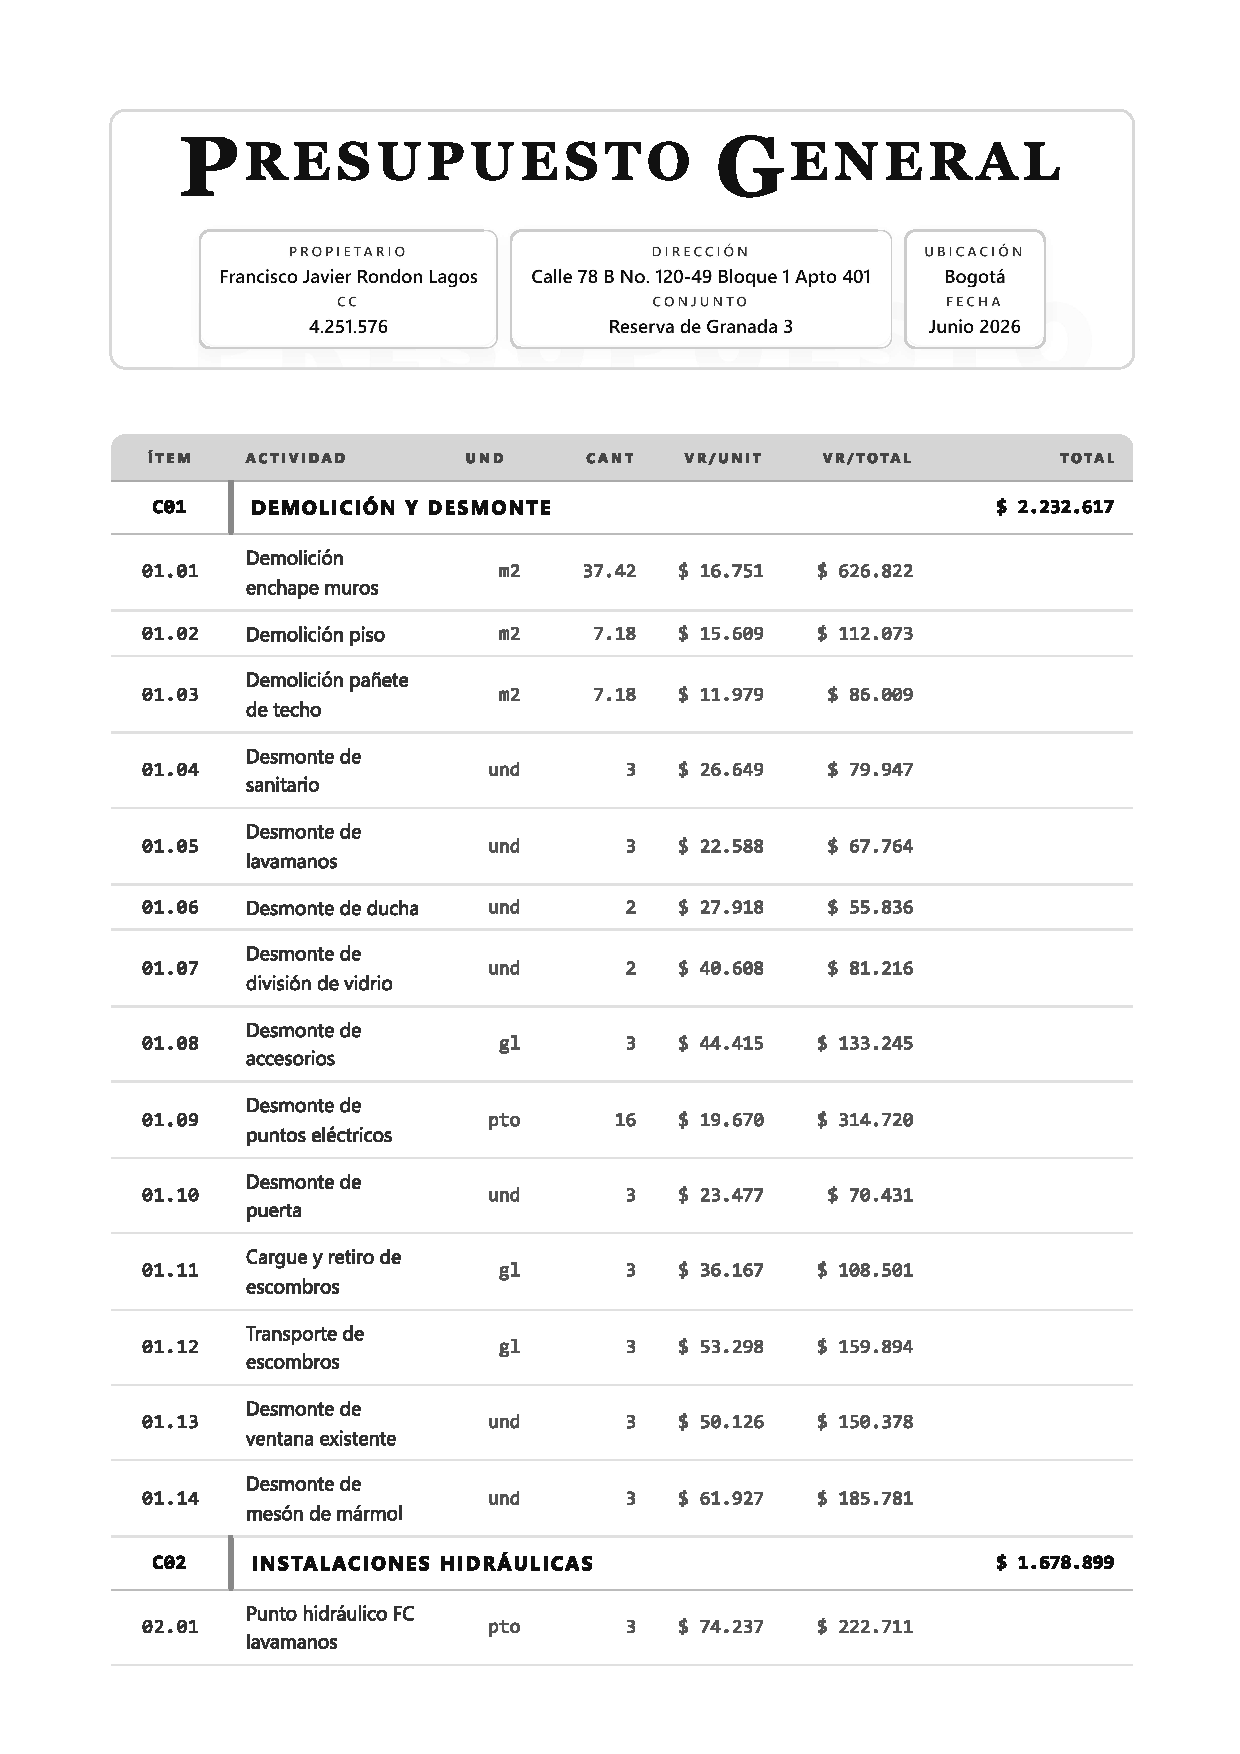
\includepdf[pages=-,pagecommand={\thispagestyle{empty}},scale=0.92,offset=0 0.5cm]{01-Presupuesto_General.pdf}
%
\newpage
\thispagestyle{plain}
\addcontentsline{toc}{part}{Anexo 1: Presupuesto General de Obra}
\vspace*{\fill}
\begin{center}
{\Huge\bfseries\color{primary}\lsstyle ANEXO 1}\\[1.2cm]
{\LARGE\bfseries\color{secondary} Presupuesto General de Obra}\\[0.6cm]
{\large\color{primary!70!black} Rehabilitación Integral de Tres Áreas Húmedas}
\end{center}
\vspace*{\fill}
\newpage
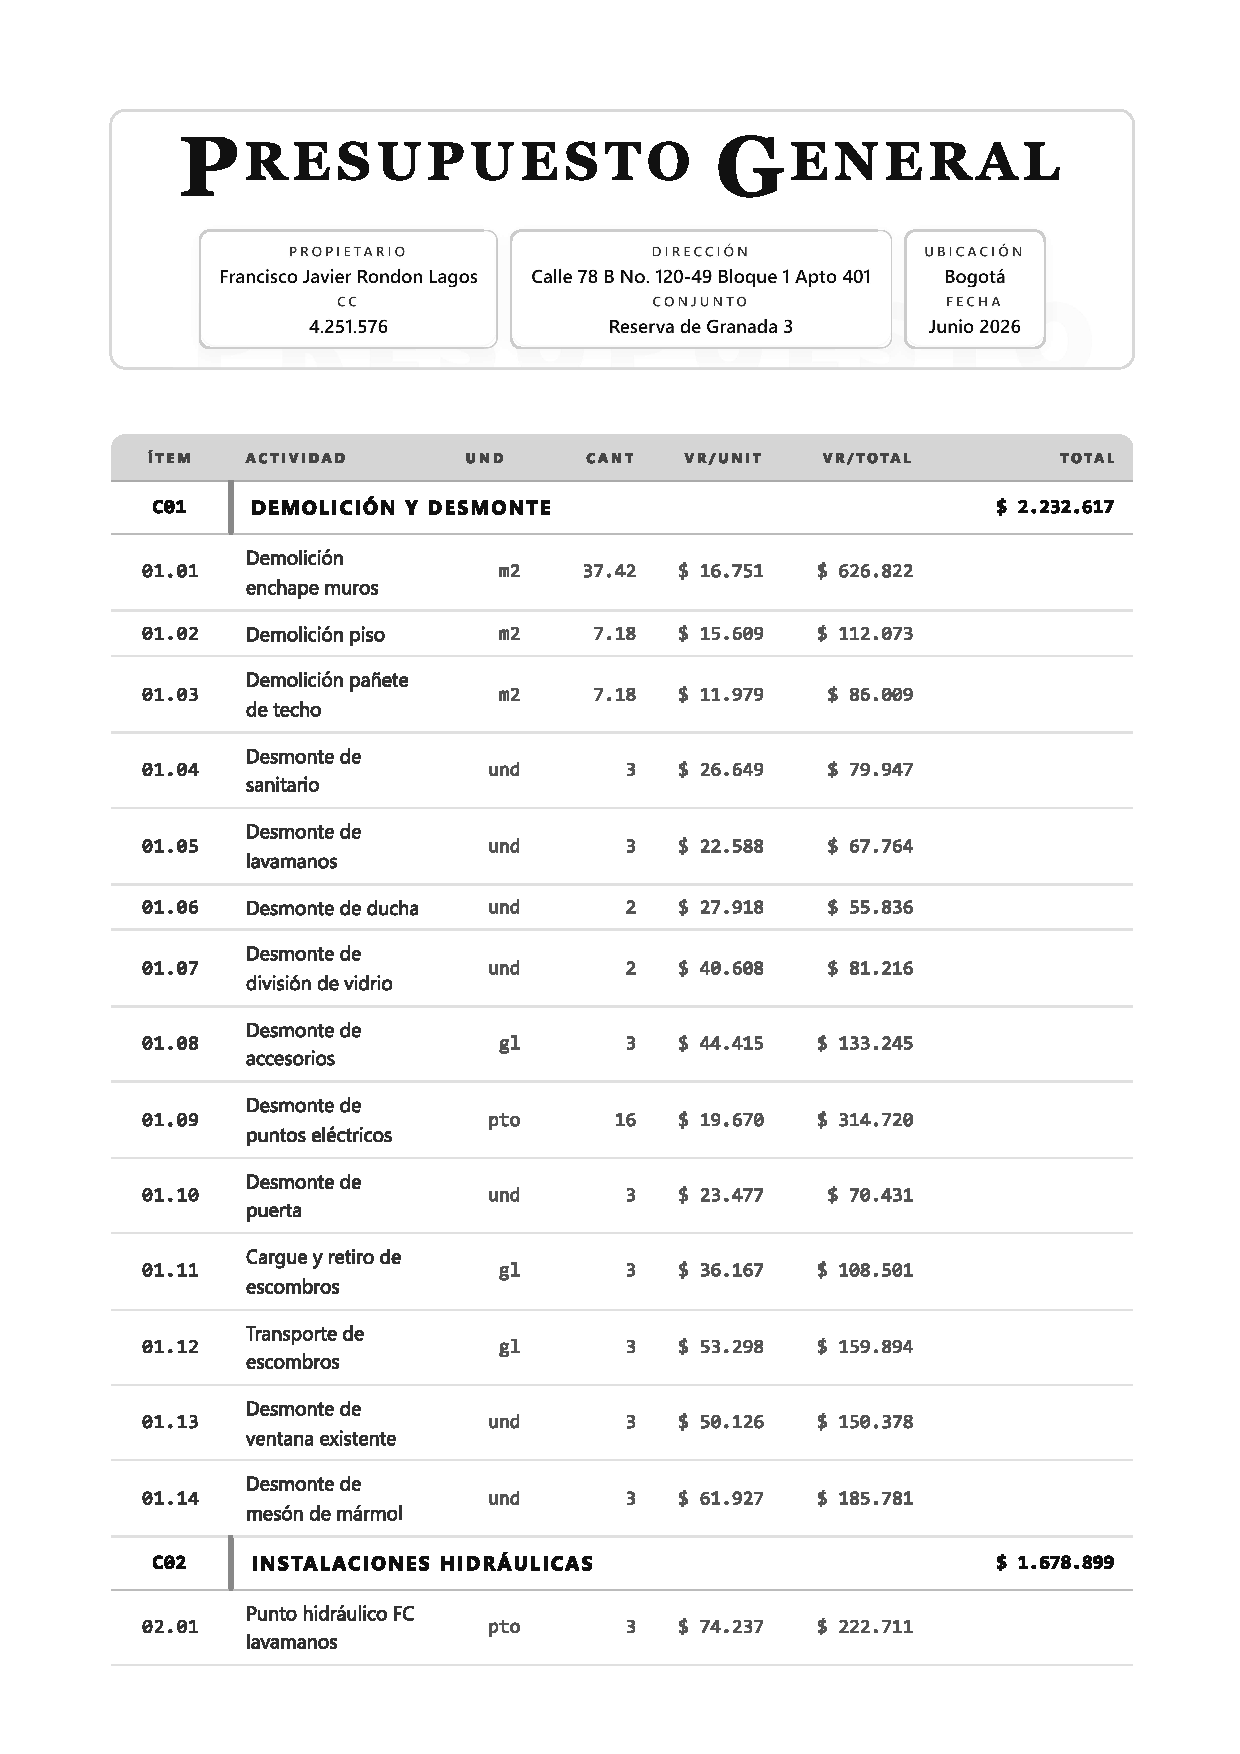
\includepdf[pages=-,pagecommand={\thispagestyle{plain}},scale=0.92,offset=0 0.5cm]{01-Presupuesto_General.pdf}
%
\newpage
\thispagestyle{plain}
\addcontentsline{toc}{part}{Anexo 2: APU Detallados por Actividad}
\vspace*{\fill}
\begin{center}
{\Huge\bfseries\color{primary}\lsstyle ANEXO 2}\\[1.2cm]
{\LARGE\bfseries\color{secondary} APU Detallados por Actividad}\\[0.6cm]
{\large\color{primary!70!black} Rehabilitación Integral de Tres Áreas Húmedas}
\end{center}
\vspace*{\fill}
\newpage
\includepdf[pages=-,pagecommand={\thispagestyle{plain}},scale=0.90,offset=0 0.5cm]{02-APUs_Detallados.pdf}
%
\newpage
\thispagestyle{plain}
\addcontentsline{toc}{part}{Anexo 3: Catálogo de Insumos}
\vspace*{\fill}
\begin{center}
{\Huge\bfseries\color{primary}\lsstyle ANEXO 3}\\[1.2cm]
{\LARGE\bfseries\color{secondary} Catálogo de Insumos}\\[0.6cm]
{\large\color{primary!70!black} Rehabilitación Integral de Tres Áreas Húmedas}
\end{center}
\vspace*{\fill}
\newpage
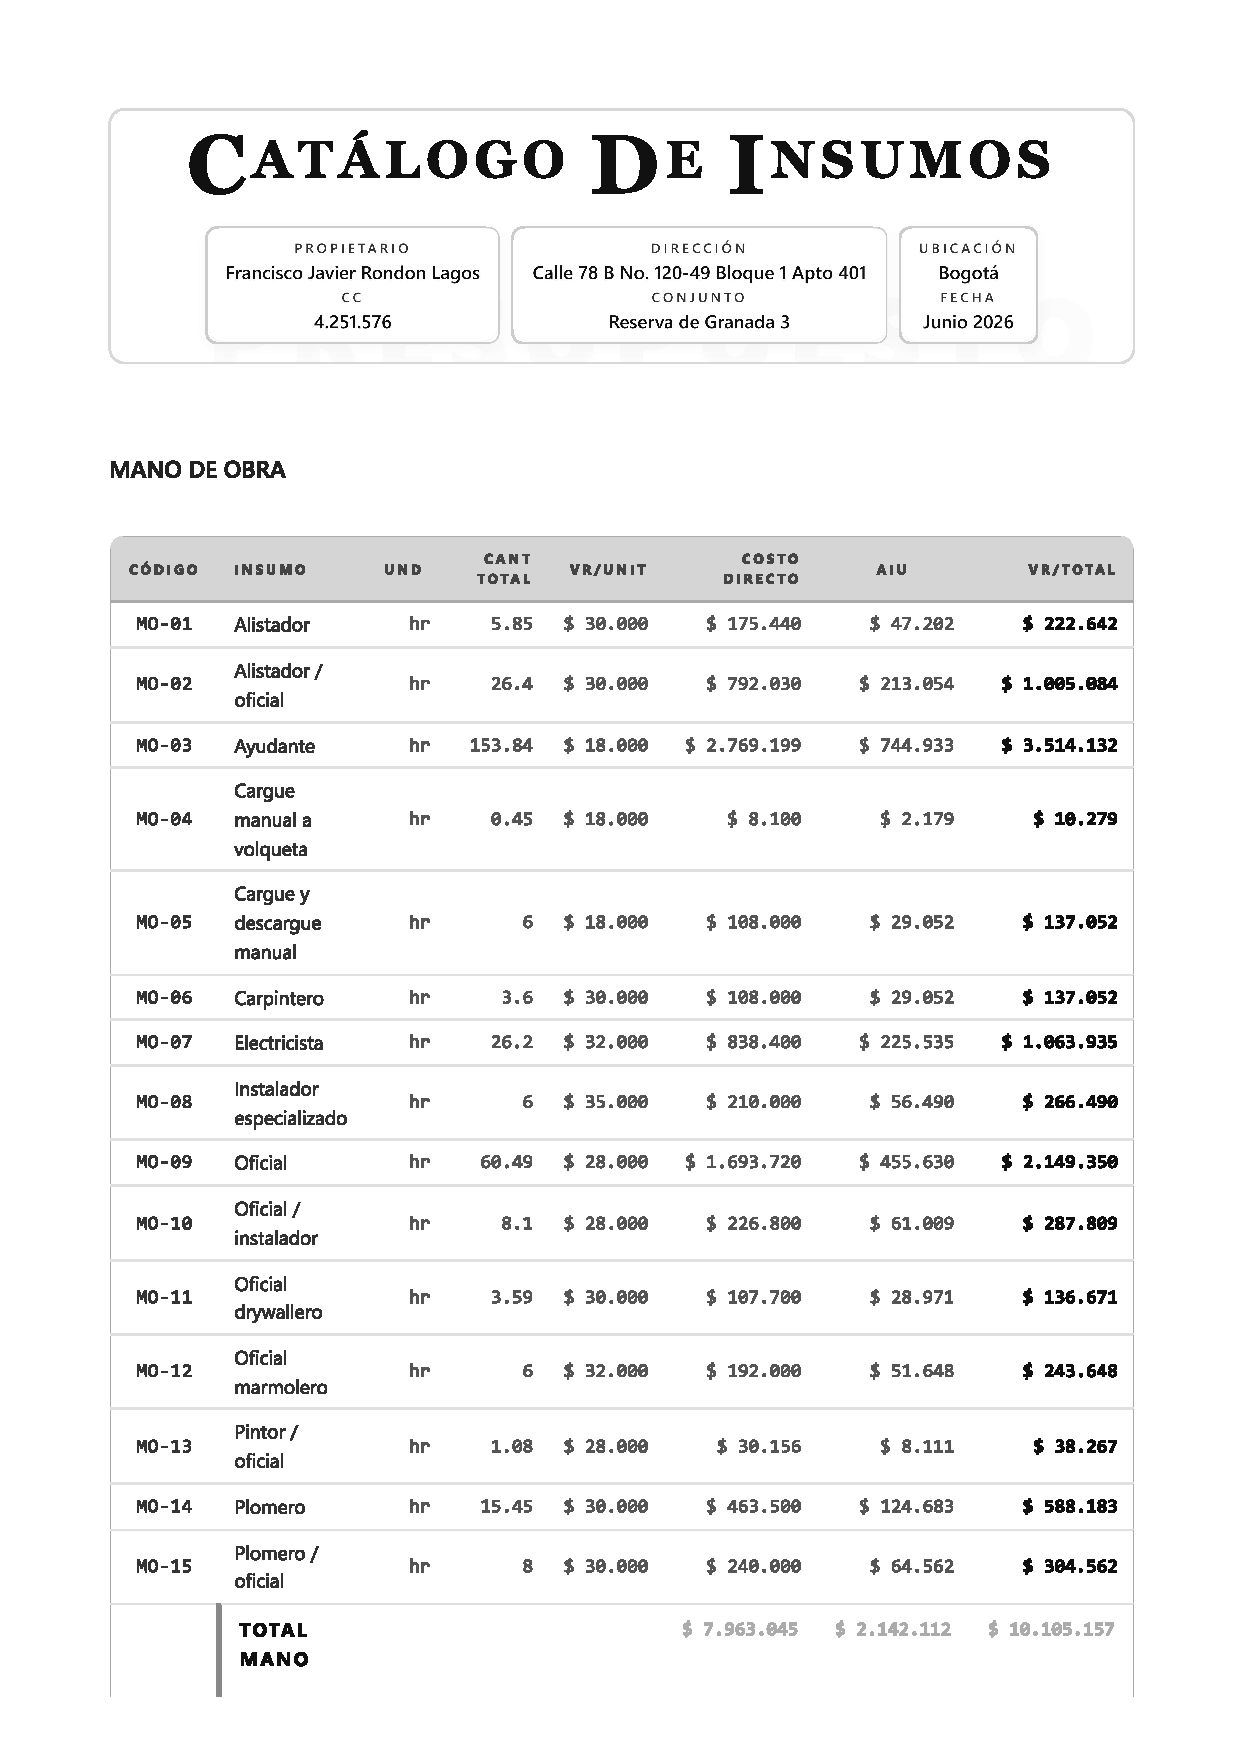
\includepdf[pages=-,pagecommand={\thispagestyle{plain}},scale=0.90,offset=0 0.5cm]{03-Insumos.pdf}
%
\newpage
\thispagestyle{plain}
\addcontentsline{toc}{part}{Anexo 4: Memoria de Cantidades de Obra}
\vspace*{\fill}
\begin{center}
{\Huge\bfseries\color{primary}\lsstyle ANEXO 4}\\[1.2cm]
{\LARGE\bfseries\color{secondary} Memoria de Cantidades de Obra}\\[0.6cm]
{\large\color{primary!70!black} Rehabilitación Integral de Tres Áreas Húmedas}
\end{center}
\vspace*{\fill}
\newpage
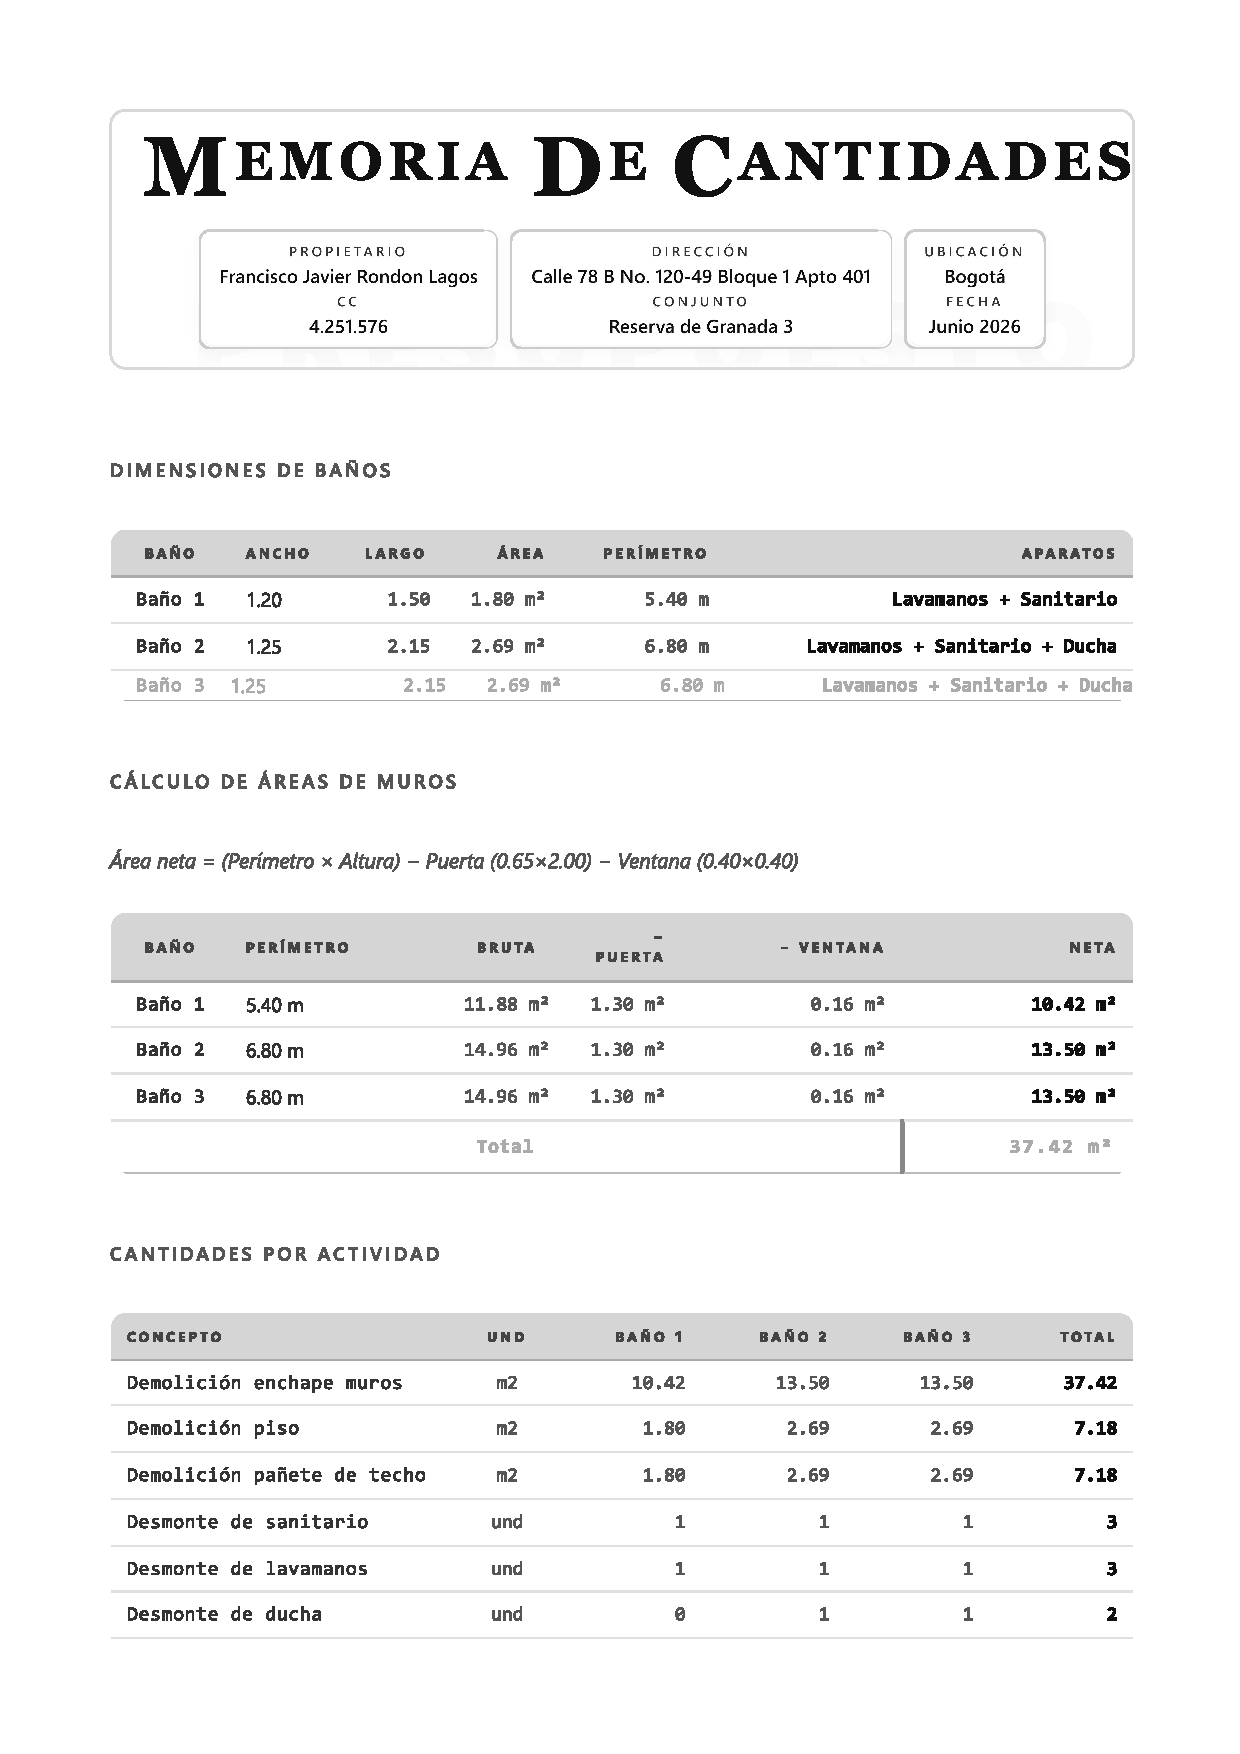
\includepdf[pages=-,pagecommand={\thispagestyle{plain}},scale=0.90,offset=0 0.5cm]{04-Memoria_Cantidades.pdf}
%
\newpage
\thispagestyle{plain}
\addcontentsline{toc}{part}{Anexo 5: Especificaciones Técnicas por Capítulo}
\vspace*{\fill}
\begin{center}
{\Huge\bfseries\color{primary}\lsstyle ANEXO 5}\\[1.2cm]
{\LARGE\bfseries\color{secondary} Especificaciones Técnicas por Capítulo}\\[0.6cm]
{\large\color{primary!70!black} Rehabilitación Integral de Tres Áreas Húmedas}
\end{center}
\vspace*{\fill}
\newpage
\includepdf[pages=-,pagecommand={\thispagestyle{plain}},scale=0.92,offset=0 0.5cm]{05-Especificaciones_Tecnicas.pdf}

\newpage
\part*{Bibliograf\'{\i}a}
\addcontentsline{toc}{part}{Bibliograf\'{\i}a}

\begin{thebibliography}{99}

\bibitem{nsr10} Ministerio de Vivienda, Ciudad y Territorio. \textit{Reglamento Colombiano de Construcción Sismo Resistente NSR-10}. Ley 1796 de 2016. Bogot\'a, Colombia.

\bibitem{retie} Ministerio de Minas y Energ\'{\i}a. \textit{Reglamento Técnico de Instalaciones Eléctricas RETIE}. Resoluci\'on 90708 de 2013. Bogot\'a, Colombia.

\bibitem{ras2000} Ministerio de Desarrollo Econ\'omico. \textit{Reglamento Técnico del Sector de Agua Potable y Saneamiento Básico RAS 2000}. Resoluci\'on 1096 de 2000. Bogot\'a, Colombia.

\bibitem{ntc2050} ICONTEC. \textit{NTC 2050: Código Eléctrico Colombiano}. Instituto Colombiano de Normas Técnicas y Certificación, Bogot\'a.

\bibitem{ntc1337} ICONTEC. \textit{NTC 1337: Tubería de PVC para conducción de agua}. Instituto Colombiano de Normas Técnicas y Certificación, Bogot\'a.

\bibitem{ntc541} ICONTEC. \textit{NTC 541: Tubería de CPVC para agua caliente}. Instituto Colombiano de Normas Técnicas y Certificación, Bogot\'a.

\bibitem{ntc4321} ICONTEC. \textit{NTC 4321: Baldosas cerámicas. Especificaciones y métodos de ensayo}. Instituto Colombiano de Normas Técnicas y Certificación, Bogot\'a.

\bibitem{ntc179} ICONTEC. \textit{NTC 179: Aparatos sanitarios de cerámica}. Instituto Colombiano de Normas Técnicas y Certificación, Bogot\'a.

\bibitem{ntc2186} ICONTEC. \textit{NTC 2186: Grifería para baño}. Instituto Colombiano de Normas Técnicas y Certificación, Bogot\'a.

\bibitem{ntc5618} ICONTEC. \textit{NTC 5618: Placas de yeso (drywall)}. Instituto Colombiano de Normas Técnicas y Certificación, Bogot\'a.

\bibitem{ntc3184} ICONTEC. \textit{NTC 3184: Membranas líquidas impermeabilizantes}. Instituto Colombiano de Normas Técnicas y Certificación, Bogot\'a.

\bibitem{ntc4425} ICONTEC. \textit{NTC 4425: Ventanas de aluminio}. Instituto Colombiano de Normas Técnicas y Certificación, Bogot\'a.

\bibitem{ntc1522} ICONTEC. \textit{NTC 1522: Vidrio para construcción}. Instituto Colombiano de Normas Técnicas y Certificación, Bogot\'a.

\bibitem{ntc771} ICONTEC. \textit{NTC 771: Puertas de madera}. Instituto Colombiano de Normas Técnicas y Certificación, Bogot\'a.

\bibitem{ntc2500} ICONTEC. \textit{NTC 2500: Cerrajería}. Instituto Colombiano de Normas Técnicas y Certificación, Bogot\'a.

\bibitem{ntc2491} ICONTEC. \textit{NTC 2491: Accesorios sanitarios}. Instituto Colombiano de Normas Técnicas y Certificación, Bogot\'a.

\bibitem{astmc1396} ASTM International. \textit{ASTM C1396: Standard Specification for Gypsum Board}. West Conshohocken, PA, USA.

\bibitem{astmd6083} ASTM International. \textit{ASTM D6083: Standard Specification for Liquid Applied Acrylic Coating}. West Conshohocken, PA, USA.

\bibitem{astmc1028} ASTM International. \textit{ASTM C1028: Standard Test Method for Determining Static Coefficient of Friction of Ceramic Tile}. West Conshohocken, PA, USA.

\bibitem{iso13007} International Organization for Standardization. \textit{ISO 13007: Ceramic tiles -- Grouts and adhesives}. Geneva, Switzerland.

\bibitem{ntc6106} ICONTEC. \textit{NTC 6106: Adhesivos cementosos para baldosas cerámicas}. Instituto Colombiano de Normas Técnicas y Certificación, Bogot\'a.

\bibitem{decreto1077} Ministerio de Vivienda, Ciudad y Territorio. \textit{Decreto 1077 de 2015: Por medio del cual se expide el Decreto Único Reglamentario del Sector Vivienda, Ciudad y Territorio}. Bogot\'a, Colombia.

\bibitem{res472} Ministerio de Ambiente y Desarrollo Sostenible. \textit{Resolución 0472 de 2017: Gestión de Residuos de Construcción y Demolición (RCD)}. Bogot\'a, Colombia.

\bibitem{microzonificacion} Alcald\'{\i}a Mayor de Bogot\'a. \textit{Decreto 523 de 2010: Microzonificación Sísmica de Bogot\'a D.C}. Bogot\'a, Colombia.

\bibitem{skempton} Skempton, A.W. \& MacDonald, D.H. \textit{The Allowable Settlements of Buildings}. Proceedings of the Institution of Civil Engineers, Vol. 5, 1956.

\bibitem{alfaro} Alfaro, C., et al. \textit{Caracterización geotécnica de los depósitos de arcilla de la Sabana de Bogotá}. Revista de Ingeniería, Universidad de los Andes, 2001.

\bibitem{jurin} Jurin, J. \textit{An Account of Some Experiments Shown Before the Royal Society}. Philosophical Transactions of the Royal Society of London, Vol. 30, 1717.

\bibitem{homecenter} Sodimac Colombia S.A. \textit{Homecenter Colombia -- Precios de materiales de construcción}. Catálogo comercial, junio 2026.

\bibitem{corona} Corona S.A. \textit{Línea de productos sanitarios y griferías}. Catálogo comercial, 2026.

\end{thebibliography}

\end{document}




